% You can choose whether you prefer a single or double column appendix.
% Whatever you choose, you will need to stick to it throughout the appendix.
% For double column style, comment the next line.
\onecolumn

\appendix
\begin{appendices}

\section{Acknowledgements}
\label{appendix:acknowledgements}

My sincere gratitude to all the participants who generously contributed to this research by dedicating their valuable time to respond to the questionnaires voluntarily, as well as the participants who willingly tested and interacted with prototypes created for this research for their feedback and evaluation through interviews. Additionally, I thank everyone who supported me in the data gathering and prototyping phase by providing hardware, testing, and debugging code.

Special appreciation goes to Shruti Rao Ph.D. Candidate (University of Amsterdam) for her constructive feedback and suggestions, which further expanded this research, and internal supervisor Dr. Hamed S. Alavi (University of Amsterdam), for his invaluable guidance and thought-provoking questions throughout the project. Also, my sincere appreciation to all the reviewers of this research, particularly drafts of this paper, for their insightful comments and contributions.

\section{Ethical considerations}
\label{appendix:ethical}

Before user studies and data gathering were conducted, an application to the Ethics Committee for Information Sciences (ECIS) \footnote{https://ivi.uva.nl/research/ethical-code/ethical-code.html} was made. No ethical issues were raised and the committee gave positive advice before the start of the research. All individuals participating in the questionnaire and evaluation process were obliged to confirm their voluntary involvement by carefully reading and submitting consent forms, with the assurance that they retained the right to withdraw from participation at any point without the need for explanation.

Participants were informed about the goal of the study and the structure of the interviews. To uphold confidentiality and privacy, questionnaire participation occurred anonymously, and all evaluation interview data underwent anonymization following the conclusion of the evaluation sessions. Interacting with occupants within the building and interacting with participants of the usability tests of the prototype adhered to the principles outlined in the University of Amsterdam Code of Conduct \footnote{https://www.uva.nl/en/about-the-uva/policy-and-regulations/} and Campus rules and Policies \footnote{https://extranet.uva.nl/en/content/a-z/house-rules-and-code-of-conduct/house-rules-and-code-of-conduct.html}.

\section{Domain Expert Validity}
\label{appendix:experts}

Before conducting the questionnaire, data gathering process, and interview evaluation procedures, domain experts from the Informatics Institute \footnote{https://ivi.uva.nl/} and the Digital Interactions Lab (DIL) \footnote{https://uva-dilab.com/} at the University of Amsterdam reviewed the methodology procedures. Draft versions of the questions and techniques were sent out to staff and supervisors for feedback internally. The questionnaire and interview procedure were pilot-tested internally. After several iterations then more widely distributed to occupants and opened for participation. 

\section{Data storage and archival}
\label{appendix:data}

During the research phase data collection methods, storage, and archival followed the Central guidelines for research data management (RDM) \footnote{https://rdm.uva.nl/en/introduction/rdm-introduction.html} from the University of Amsterdam. All occupant data was anonymized before publishing and nothing that can be considered personal data is collected. Data is stored on cloud service providers provided by the University of Amsterdam such as Research Drive \footnote{https://rdm.uva.nl/en/looking-after/storage/storage.html}. Only the principal researcher and supervisor(s) in possession of the encryption methods and passwords can view the unstructured exported data from the questionnaires, monitoring devices, and interviews. Only aggregated datasets and data outputs for the purpose of visualization are published and can be publicly viewed.

\section{Source code and datasets}
\label{appendix:source}

In the spirit of Open Access Research \footnote{https://uba.uva.nl/en/support/research/open-access/open-access.html}, to support reproducibility, mitigate a lack of transparency, and enable future work in this research field the aggregated datasets, notebooks, and prototype source code in this research are publicly available on a GitHub organization with the working title 'viszlab' \footnote{https://github.com/viszlab} using the MIT License. Several code repositories for different parts of the research can be accessed and publicly viewed. The README file of each repository describes the contents and how to perform the technical set-up. Notable repositories are:

\begin{enumerate}
  \item \textbf{Prototype}. Arduino Code, component diagrams, and 3D models for the physical prototype.\\
  \underline{https://github.com/viszlab/prototype}
  \item \textbf{Datasets}. Python code and notebooks for data analysis of the questionnaire, monitor devices, and evaluation.\\
  \underline{https://github.com/viszlab/prototype}
  \item \textbf{Website}. One-pager website where all outputs such as this paper and photographs of the research can be downloaded.\\
  \underline{https://github.com/viszlab/viszlab.github.io}  
\end{enumerate}

\pagebreak

\section{Floorplan and lab set-up}
\label{appendix:floorplan}

A diagram providing an overview of the technical lab-setup of the IAQ monitors

\begin{figure}[H]
    \centering
    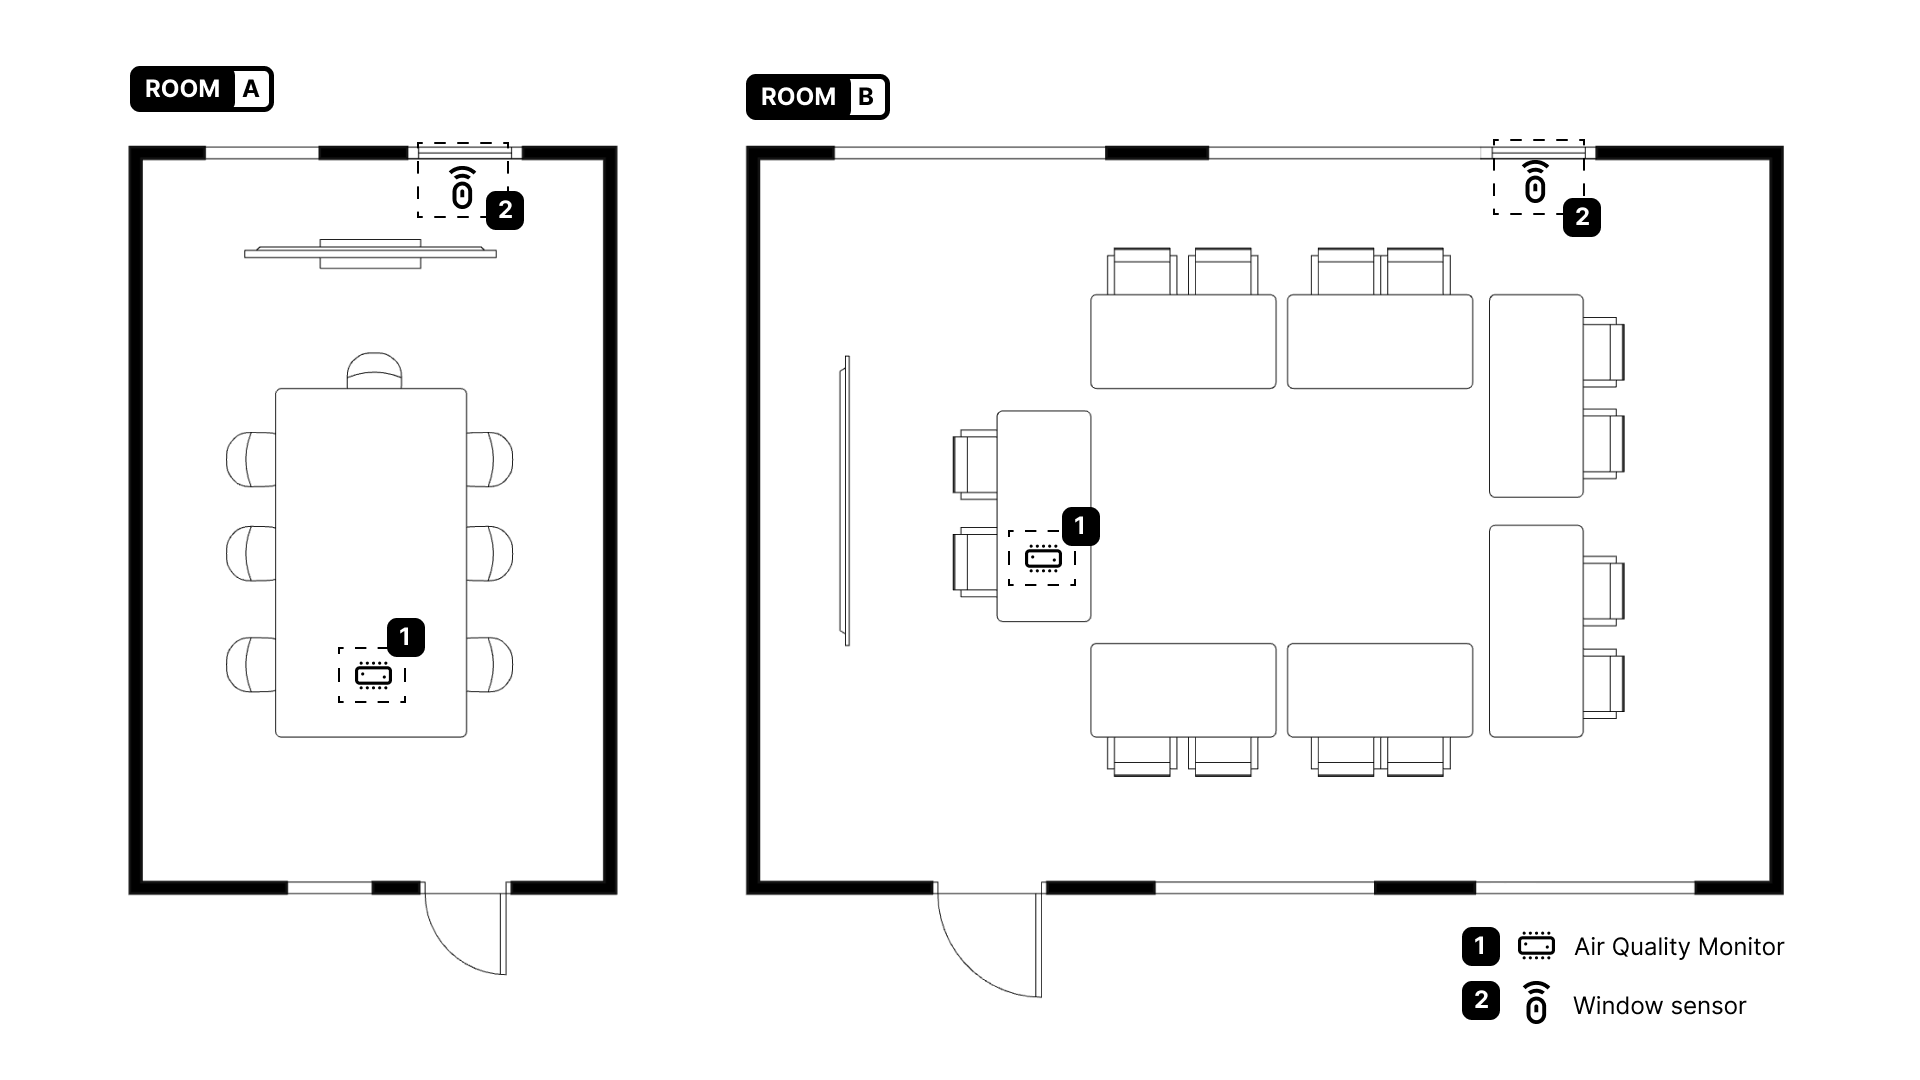
\includegraphics[width=0.8\paperwidth]{floorplan.png}
    \caption{Floorplan of Room A and B with the position of the monitor devices installed to manufacturer specifications}
    \label{fig:timeline}
\end{figure}

\section{Meeting room impressions}
\label{appendix:meetings}

Photographs of the meeting rooms used for the lab-setup.

\begin{figure}[H]
\begin{minipage}{.5\textwidth}
    \centering
    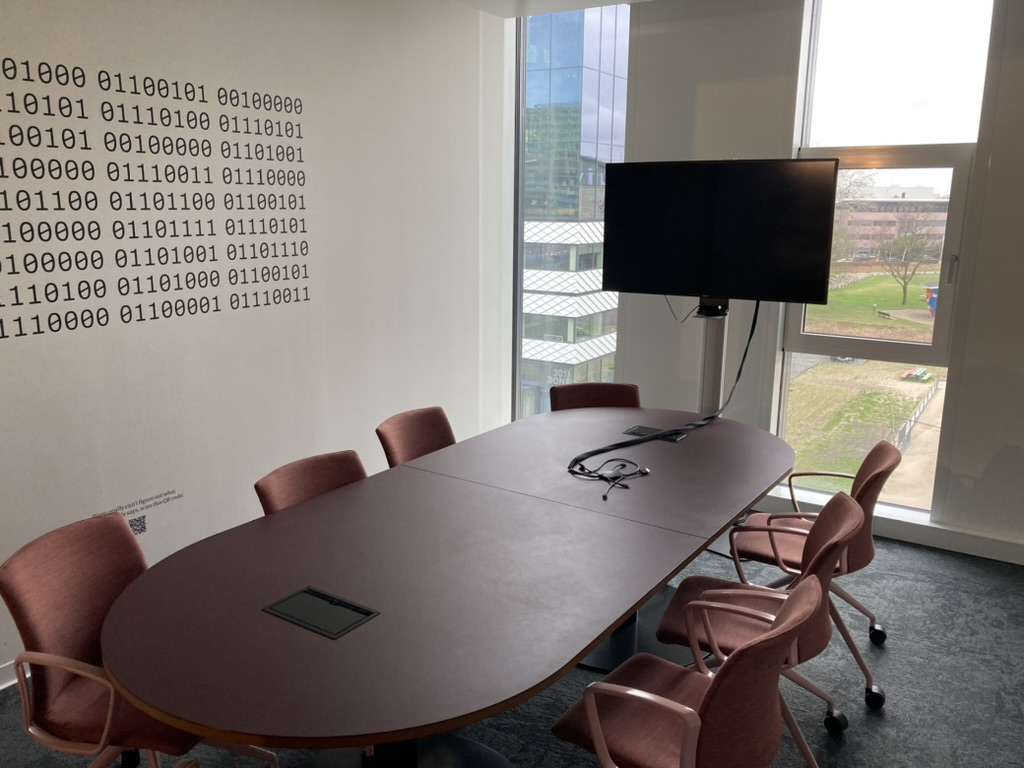
\includegraphics[width=85mm,height=70mm]{photograph-room-a.jpeg}
    \caption{The 'smaller'($m2$) space labeled Room A}
    \label{fig:timeline}
\end{minipage}%
\begin{minipage}{.5\textwidth}
    \centering
    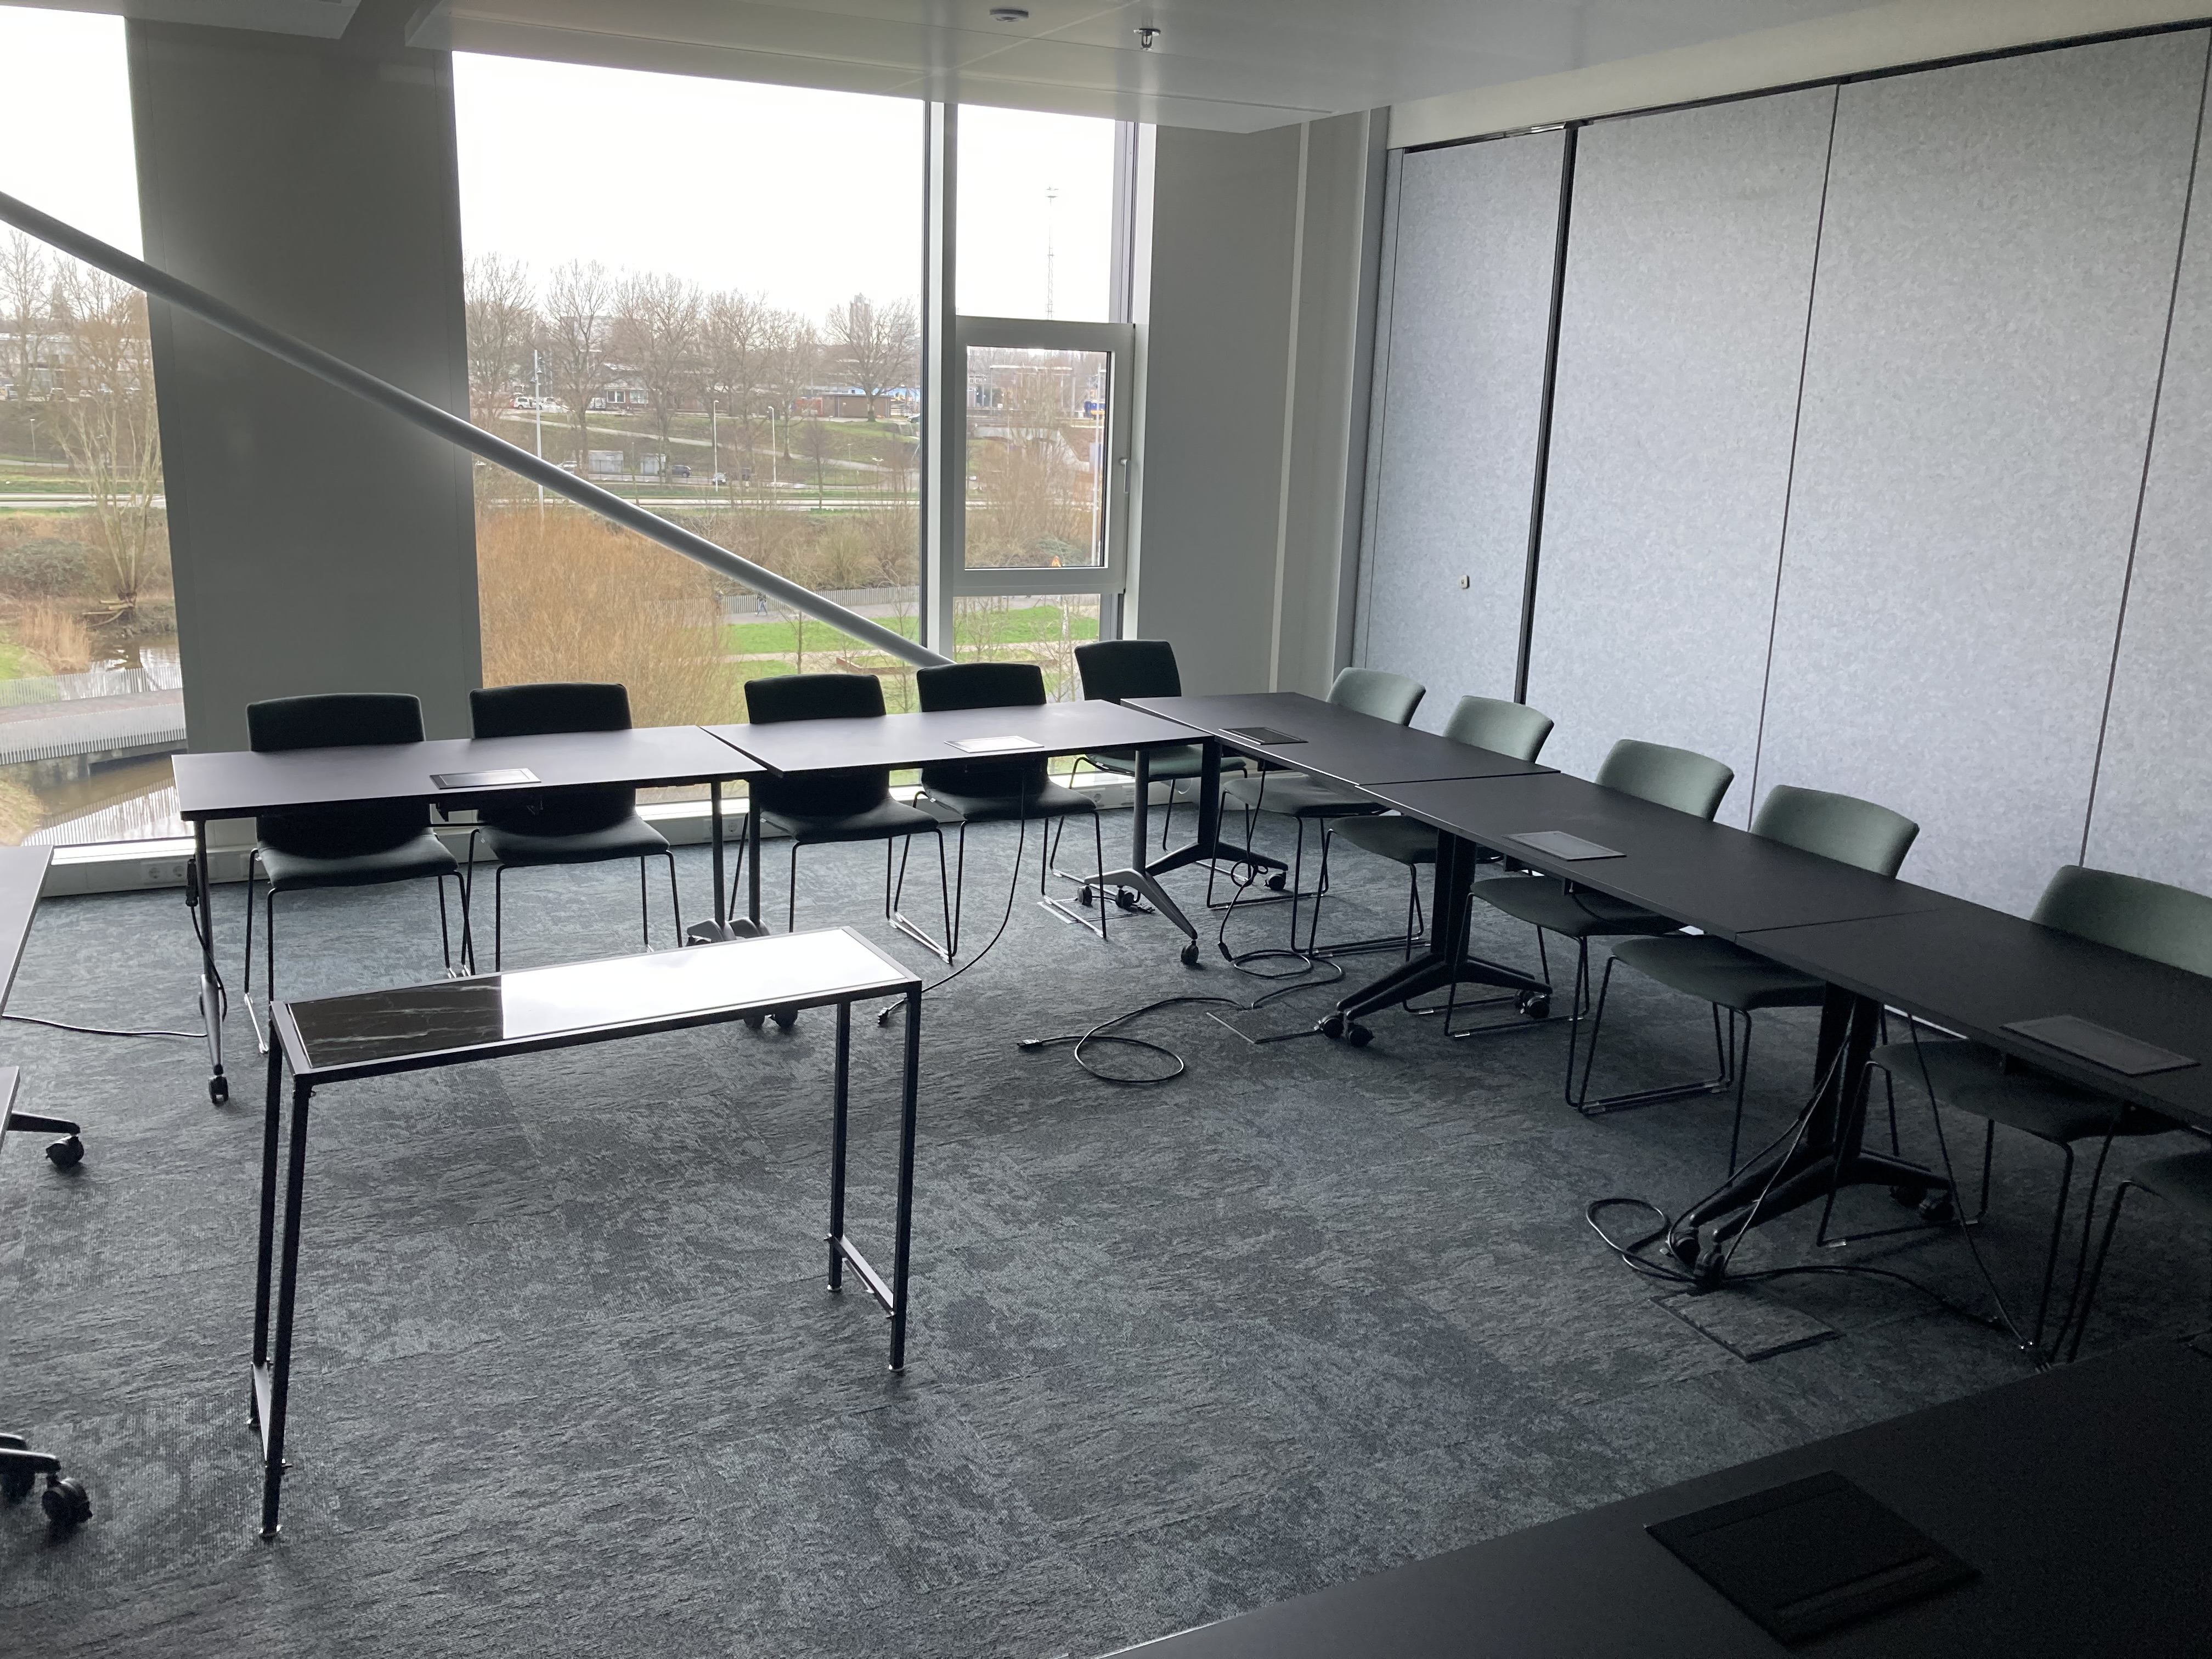
\includegraphics[width=85mm,height=70mm]{photograph-room-b.jpeg}
    \caption{The 'larger' ($m2$) space labeled Room B}
    \label{fig:timeline}
\end{minipage}%
\end{figure}

\section{Building impressions}
\label{appendix:building}

\begin{figure}[H]
\begin{minipage}{.5\textwidth}
\begin{tabular}{cc}
  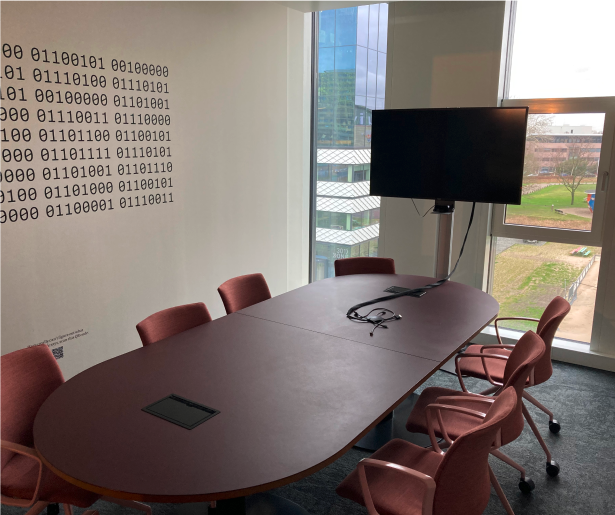
\includegraphics[width=45mm]{building.png} &   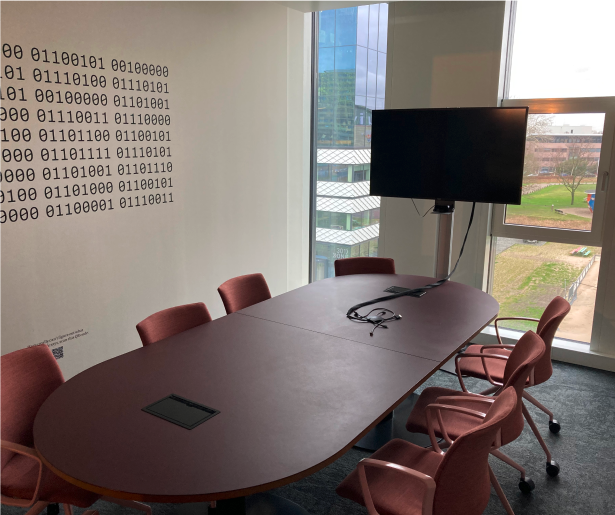
\includegraphics[width=45mm]{building.png} \\
(a) first & (b) second \\[6pt]
 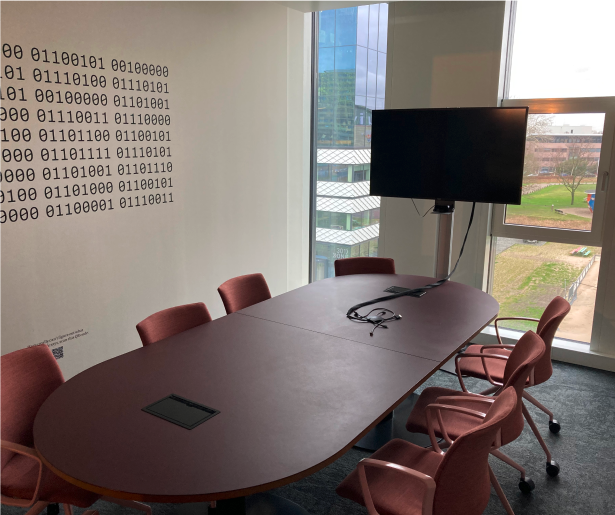
\includegraphics[width=45mm]{building.png} &   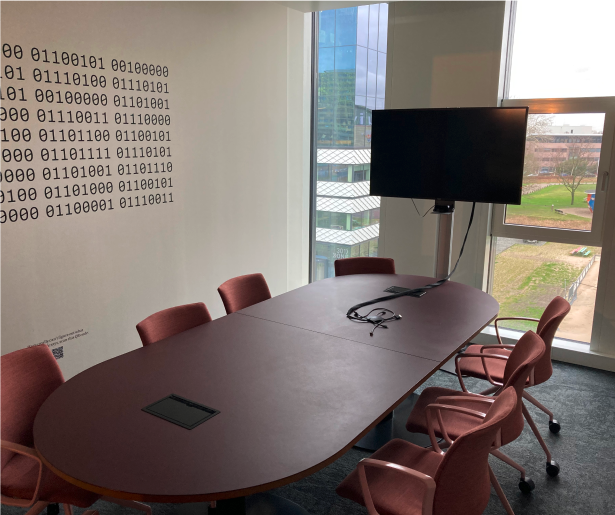
\includegraphics[width=45mm]{building.png} \\
(c) third & (d) fourth \\[6pt]
\end{tabular}
\caption{caption}
\end{minipage}%
\begin{minipage}{.5\textwidth}
    \centering
    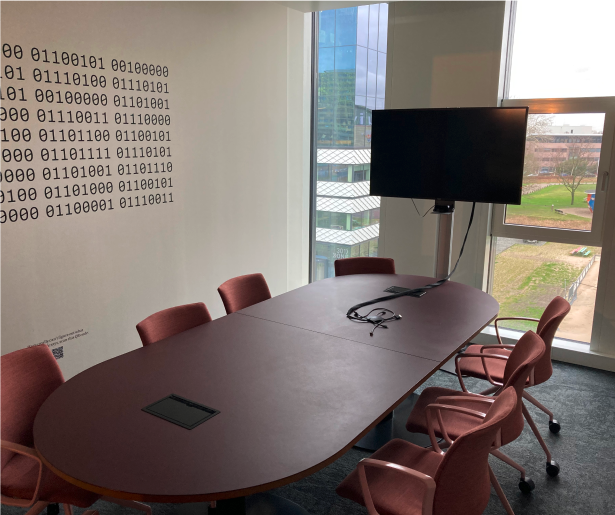
\includegraphics[width=70mm,height=80mm]{building.png}
    \caption{System diagram that shows the }
    \label{fig:timeline}
\end{minipage}%
\end{figure}

\section{Prototype impressions}
\label{appendix:prototype}

\begin{figure}[H]
\begin{minipage}{.5\textwidth}
    \centering
    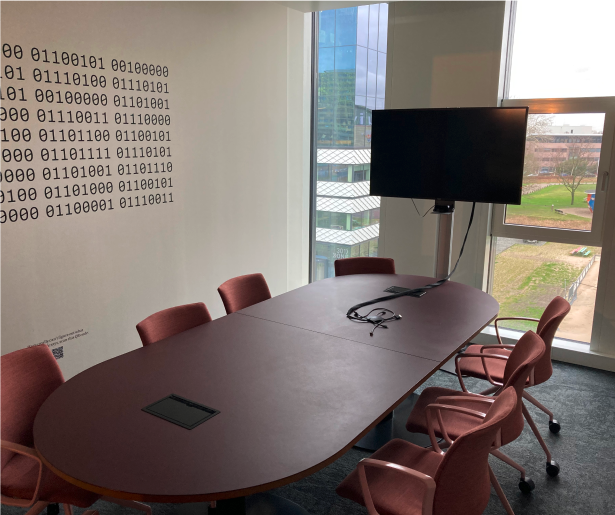
\includegraphics[width=70mm,height=80mm]{building.png}
    \caption{System diagram that shows the }
    \label{fig:timeline}
\end{minipage}%
\begin{minipage}{.5\textwidth}
\begin{tabular}{cc}
  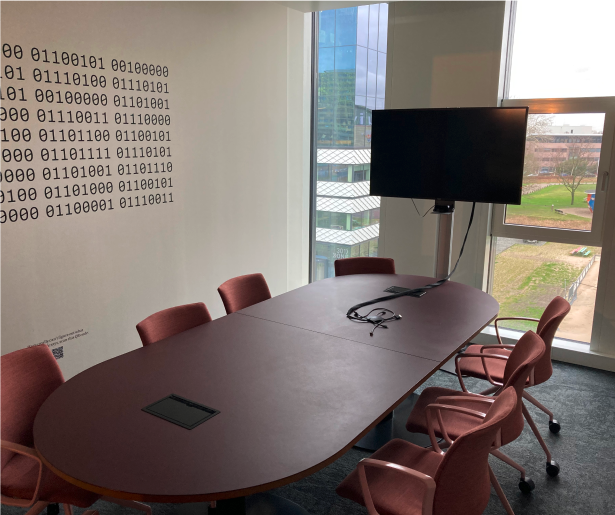
\includegraphics[width=45mm]{building.png} &   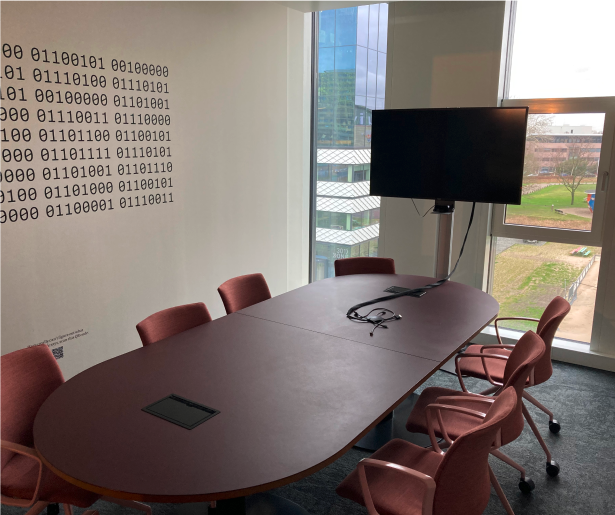
\includegraphics[width=45mm]{building.png} \\
(a) first & (b) second \\[6pt]
 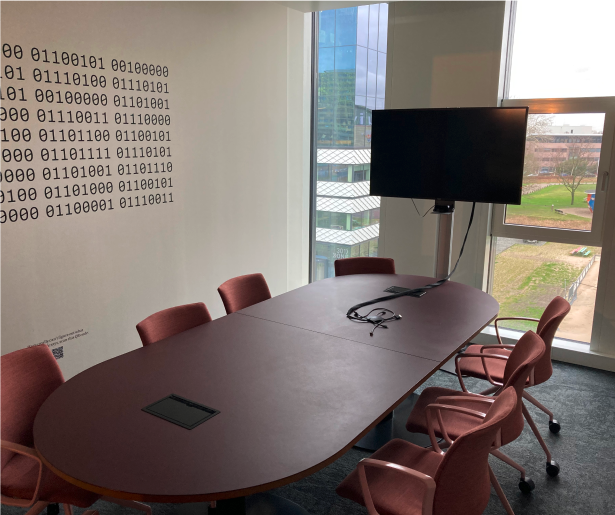
\includegraphics[width=45mm]{building.png} &   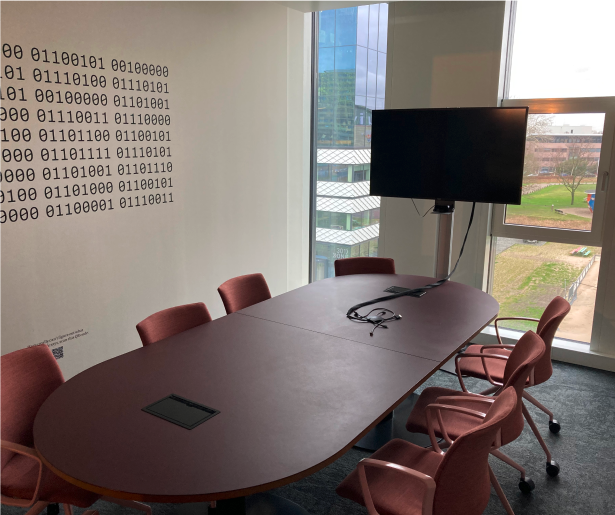
\includegraphics[width=45mm]{building.png} \\
(c) third & (d) fourth \\[6pt]
\end{tabular}
\caption{caption}
\end{minipage}%
\end{figure}

\section{IoT architecture of the prototype}
\label{appendix:architecture}

System diagram which shows the IoT architecture of the prototype.

\begin{figure}[H]
    \centering
    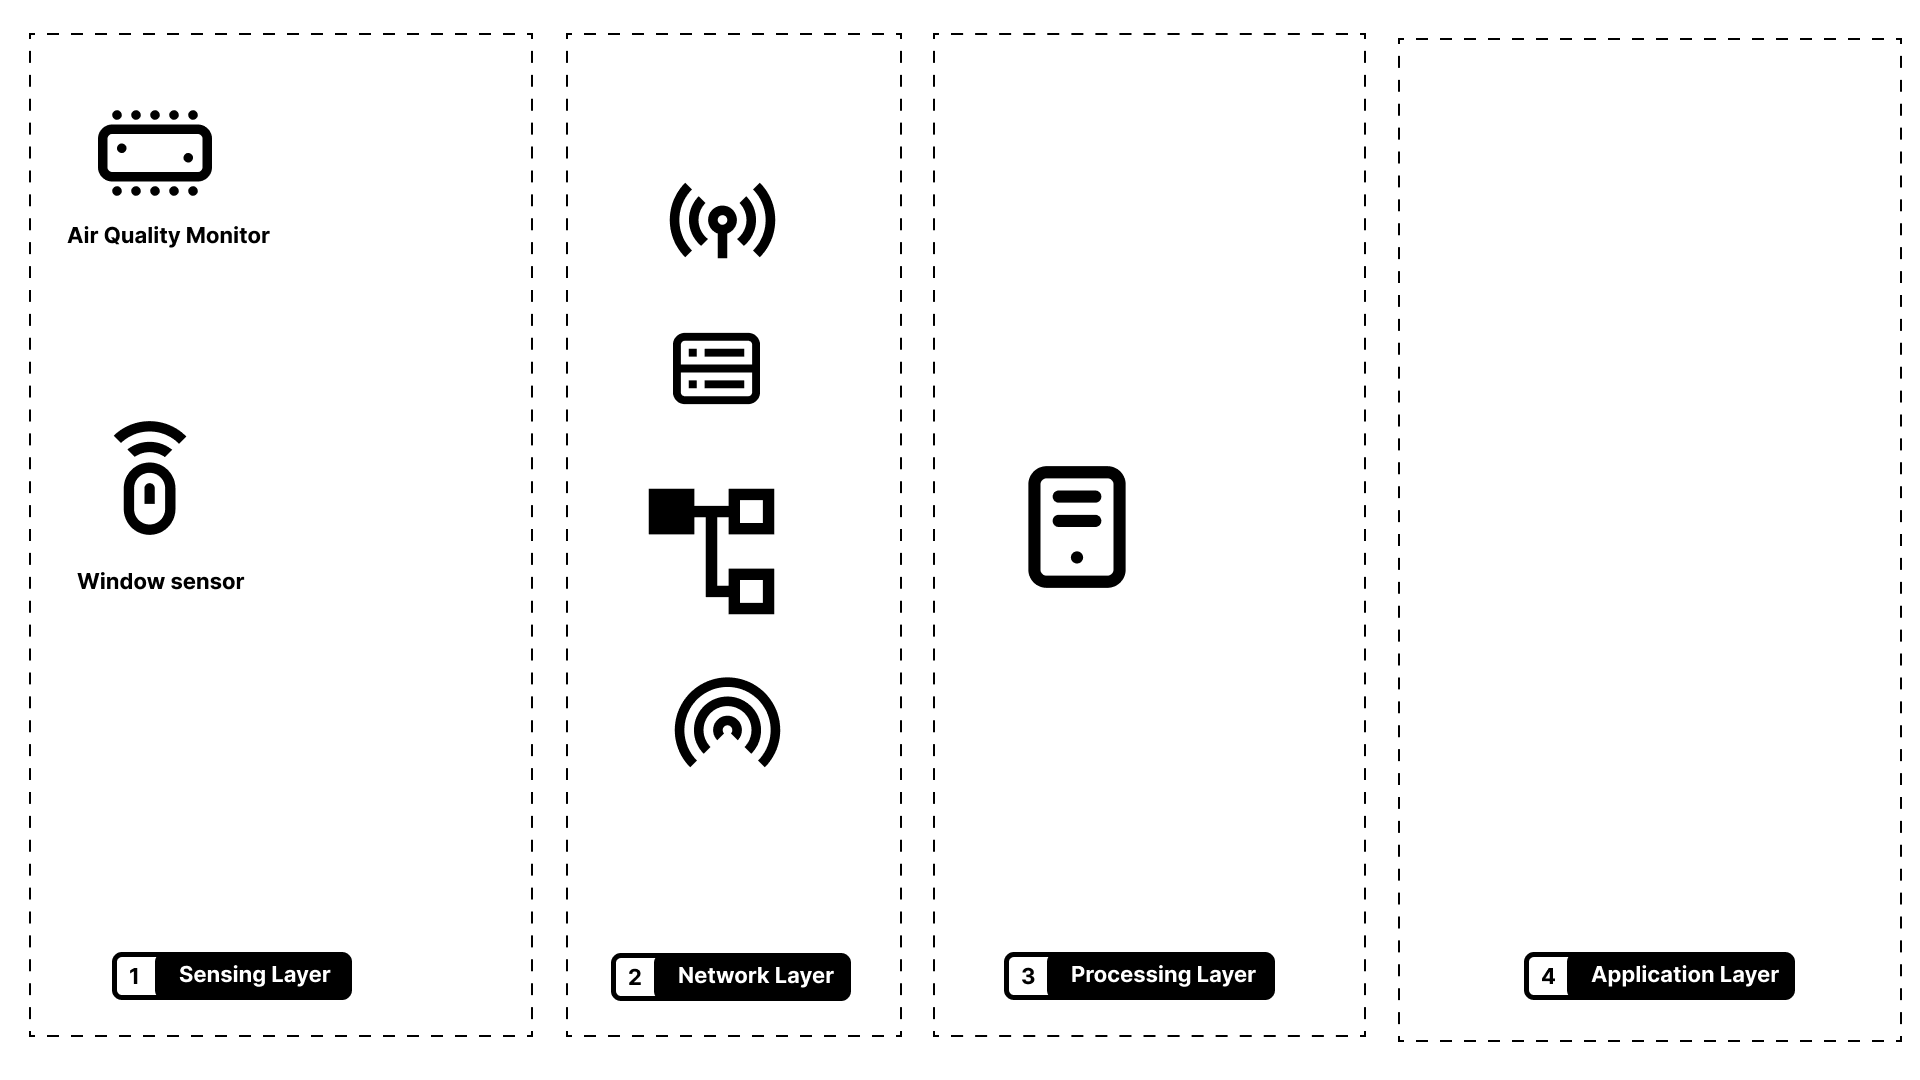
\includegraphics[width=0.7\paperwidth]{system.png}
    \caption{System diagram that shows the technical set-up of the prototype}
    \label{fig:timeline}
\end{figure}

\section{Existing Building API sample data}
\label{appendix:architecture}

Overview of the current building API with outputs.

\begin{figure}[H]
    \centering
    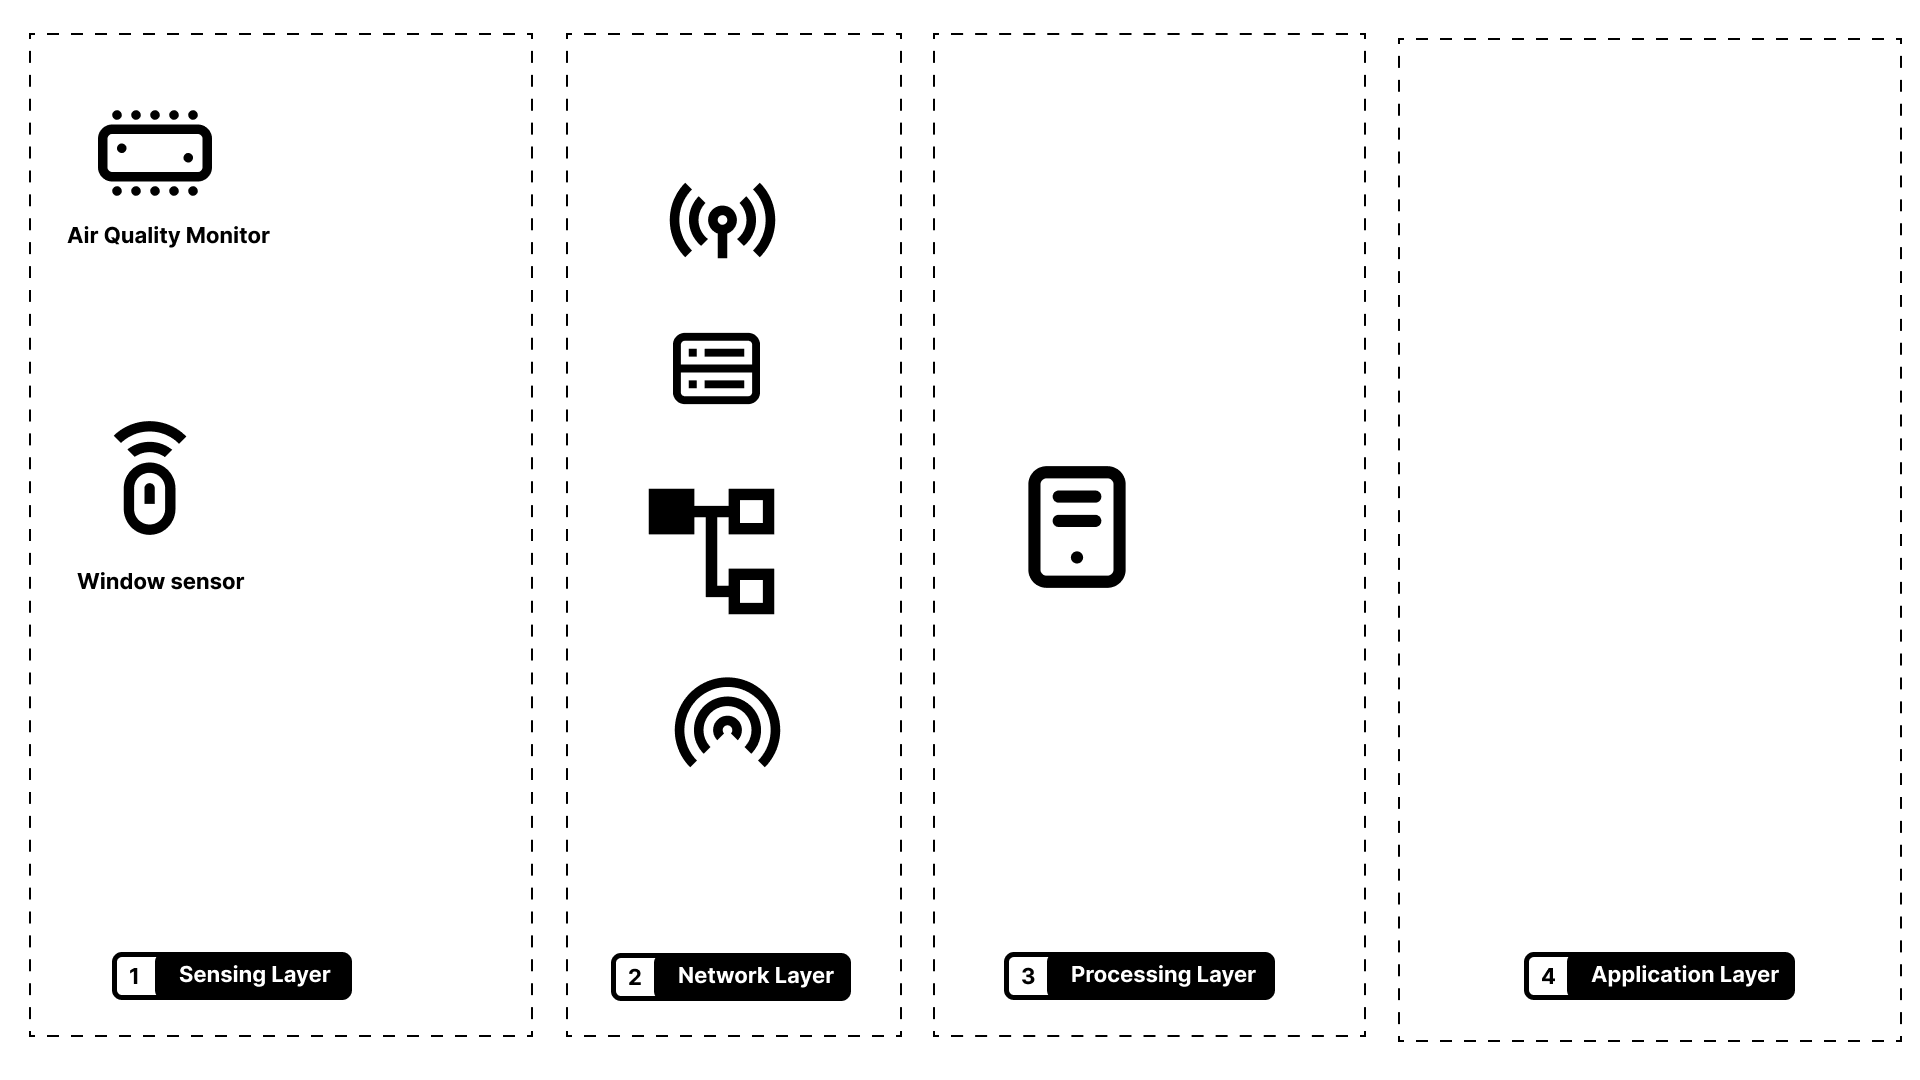
\includegraphics[width=0.7\paperwidth]{system.png}
    \caption{System diagram that shows the technical set-up of the prototype}
    \label{fig:timeline}
\end{figure}

\section{Air Quality Monitors sample data}
\label{appendix:monitors}

Sample data log of the monitor devices.

\begin{table}[H]
    \centering
    \resizebox{\textwidth}{!}{%
    \tiny
    \begin{tabular}{@{} *{11}{c} @{}}
        \toprule
        \textbf{Date} & \textbf{Time} & \textbf{CO2} & \textbf{Temp} & \textbf{RH} & \textbf{PM1.0} & \textbf{PM2.5} & \textbf{PM10} & \textbf{TVOC} & \textbf{BP} & \textbf{O3} \\
        \midrule
        2024/04/03 & 10:30 & 647 & 21'C & 39\% & 0 & 0 & 0 & 255 & 99.97 & 0 \\
        2024/04/03 & 10:29 & 641 & 21'C & 39\% & 0 & 0 & 0 & 249 & 99.97 & 0 \\
        2024/04/03 & 10:28 & 633 & 21'C & 39\% & 0 & 0 & 0 & 246 & 99.97 & 0 \\
        2024/04/03 & 10:27 & 635 & 21'C & 39\% & 1 & 1 & 1 & 242 & 99.97 & 0 \\
        2024/04/03 & 10:26 & 632 & 21'C & 39\% & 0 & 1 & 1 & 237 & 99.97 & 0 \\
        2024/04/03 & 10:25 & 628 & 21'C & 39\% & 0 & 1 & 1 & 236 & 99.97 & 0 \\
        2024/04/03 & 10:24 & 617 & 21'C & 39\% & 0 & 1 & 1 & 232 & 99.97 & 0 \\
        2024/04/03 & 10:23 & 602 & 21'C & 39\% & 0 & 1 & 1 & 232 & 99.97 & 0 \\
        2024/04/03 & 10:22 & 598 & 21'C & 39\% & 0 & 0 & 0 & 231 & 99.97 & 0 \\
        2024/04/03 & 10:21 & 591 & 21'C & 39\% & 0 & 1 & 1 & 228 & 99.97 & 0 \\
        2024/04/03 & 10:20 & 587 & 21'C & 39\% & 0 & 0 & 0 & 228 & 99.97 & 0 \\
        2024/04/03 & 10:19 & 580 & 21'C & 39\% & 0 & 0 & 0 & 230 & 99.97 & 0 \\
        2024/04/03 & 10:18 & 580 & 21'C & 39\% & 0 & 0 & 0 & 232 & 99.97 & 0 \\
        2024/04/03 & 10:17 & 578 & 21'C & 39\% & 1 & 1 & 1 & 234 & 99.97 & 0 \\
        2024/04/03 & 10:16 & 574 & 21'C & 39\% & 0 & 0 & 0 & 237 & 99.97 & 0 \\
        2024/04/03 & 10:15 & 569 & 21'C & 39\% & 0 & 0 & 0 & 237 & 99.97 & 0 \\
        \bottomrule
    \end{tabular}%
    }
    \vspace{10pt} % Adjust the amount of whitespace as needed
    \caption{Sample data log of the Aircheq Touch Aero installed in the 'small' Room A} 
    \label{tab:room-A}
\end{table}

\begin{table}[H]
    \centering
    \resizebox{\textwidth}{!}{%
    \tiny
    \begin{tabular}{@{} *{11}{c} @{}}
        \toprule
        \textbf{Date} & \textbf{Time} & \textbf{Temp} & \textbf{RH} & \textbf{DewPoint} & \textbf{CO2} & \textbf{-} & \textbf{-} & \textbf{-} & \textbf{-} & \textbf{-} \\
        \midrule
        10/04/2024 & 14:17:00 & 21.019 & 30.780 & 3.176 & 871.000 \\
        10/04/2024 & 14:18:00 & 21.039 & 30.573 & 3.098 & 871.000 \\
        10/04/2024 & 14:19:00 & 21.019 & 30.365 & 2.985 & 827.000 \\
        10/04/2024 & 14:20:00 & 21.049 & 30.164 & 2.917 & 808.000 \\
        10/04/2024 & 14:21:00 & 21.059 & 29.895 & 2.838 & 808.000 \\
        10/04/2024 & 14:22:00 & 21.059 & 29.852 & 2.772 & 773.000 \\
        10/04/2024 & 14:23:00 & 21.059 & 29.730 & 2.723 & 773.000 \\
        10/04/2024 & 14:24:00 & 21.079 & 29.608 & 2.665 & 773.000 \\
        10/04/2024 & 14:25:00 & 21.059 & 29.486 & 2.607 & 721.000 \\
        10/04/2024 & 14:26:00 & 21.059 & 29.303 & 2.520 & 714.000 \\
        10/04/2024 & 14:27:00 & 21.049 & 29.242 & 2.482 & 714.000 \\
        10/04/2024 & 14:28:00 & 21.079 & 29.181 & 2.479 & 714.000 \\
        10/04/2024 & 14:29:00 & 21.059 & 29.016 & 2.400 & 681.000 \\
        10/04/2024 & 14:30:00 & 21.089 & 28.912 & 2.358 & 681.000 \\
        \bottomrule
    \end{tabular}%
    }\vspace{10pt} % Adjust the amount of whitespace as needed
    \caption{Sample data log of the Atal ATU-CT ClimaTrend installed in the 'large' Room B} 
    \label{tab:room-b}
\end{table}


\section{Questionnaire survey (POE)}
\label{appendix:survey}

Exported text version of the questionnaire survey created in Qualtrics and distributed using handouts on QR codes.

\vspace{10pt} % Adjust the length as needed

\textbf{Introduction:}
\textit{Hi! We at the Digital Interactions Lab (DIL) are researching indoor environments, focusing on Indoor Air Quality (IAQ) within smart buildings like Lab42, for a Master Thesis. This survey takes an average of $\sim$3 minutes to complete and comprises questions about your overall comfort and awareness of Indoor Air Quality (IAQ).}\\

\textbf{Informed Consent:}
\textit{The survey is anonymous and collects data on environmental experiences and approximate building location for future research and publication. Participation is voluntary, and if you decide that you do not want to participate after you have completed it, please contact us. Principal researcher: BSc D. de Vries - danny.de.vries@student.uva.nl Supervisor(s): Shruti Rao PhD Candidate - s.rao@uva.nl Supervisor(s): Dr. H. Seiied Alavi PhD - ha.alavi@uva.nl Thank you for your valuable time and for participating in our survey!}

\vspace{10pt} % Adjust the length as needed

\textbf{Q1: Location}- Where are you currently located within the Lab42 building? \textit{Multiple-choice, one option possible}

\begin{itemize}
    \item On the ground floor (the atrium)
    \item On the first floor (1st floor - in a working space)
    \item On the second floor (2nd floor - in a working space)
\end{itemize}

\textbf{Q2: Activity} - On average, how often do you use Lab42 per week for various activities? \textit{Multiple-choice, one option possible}

\begin{itemize}
    \item 1 day a week
    \item 2 days a week
    \item 3 days a week
    \item 4 days a week
    \item 5 days a week
\end{itemize}

\textbf{Q3: Occupancy} - How would you describe the occupancy in your current space? \textit{Multiple-choice, one option possible}

\begin{itemize}
    \item Not crowded
    \item Not too crowded
    \item Crowded
    \item Very crowded
    \item At capacity
\end{itemize}

\textbf{Q4: Awareness Air Quality} - Did you know that poor air quality has been identified to pose health risks and affect cognitive performance? How aware are you of the current air quality in this space? \textit{Likert-scale, one option possible}

\textbf{1)} Very Unaware \textbf{2)} Unaware \textbf{3)} Neutral \textbf{4)} Aware \textbf{5)} Very Aware

\vspace{10pt}

\textbf{Q6: Perceived Air Quality} - How do you perceive the air quality in the current space? \textit{Likert-scale, one option possible}

\textbf{1)} Very Poor \textbf{2)} Poor \textbf{3)} Acceptable \textbf{4)} Good \textbf{5)} Very Good 

\vspace{10pt}

\textbf{Q7: Satisfaction Air Quality} - How satisfied are you with the air quality in the current space? \textit{Likert-scale, one option possible}

\textbf{1)} Very Dissatisfied \textbf{2)} Dissastisfied \textbf{3)} Neither dissatisfied or satisfied \textbf{4)} Satisfied \textbf{5)} Very Satisfied

\vspace{10pt}

\textbf{Q8: Not mandatory} - Would you like to describe in more detail in your own words how you currently feel about the Indoor Air Quality? \textit{Open-question, insert text}

\vspace{10pt}

\textbf{Q9: Health symptoms} - Do you experience any health-related symptoms based on the air quality in this space? \textit{Multiple-choice, multiple options possible, insert text field}

\begin{itemize}
    \item None
    \item Headaches
    \item Trouble breathing
    \item Feeling nauseating
    \item Other
\end{itemize}

\textbf{Q10: Cognitive symptoms} - Do you experience any cognitive-based symptoms on the air quality in this space? \textit{Multiple-choice, multiple options possible, insert text field}

\begin{itemize}
    \item None
    \item Trouble with focus
    \item Decreased productivity
    \item Tiredness
    \item Other
\end{itemize}


\section{Survey data}
\label{appendix:survey-data}

Plots of the results of the survey data exported from Qualtrics.

\begin{figure}[htbp]
    \centering
    \begin{subfigure}{0.4\textwidth}
        \centering
        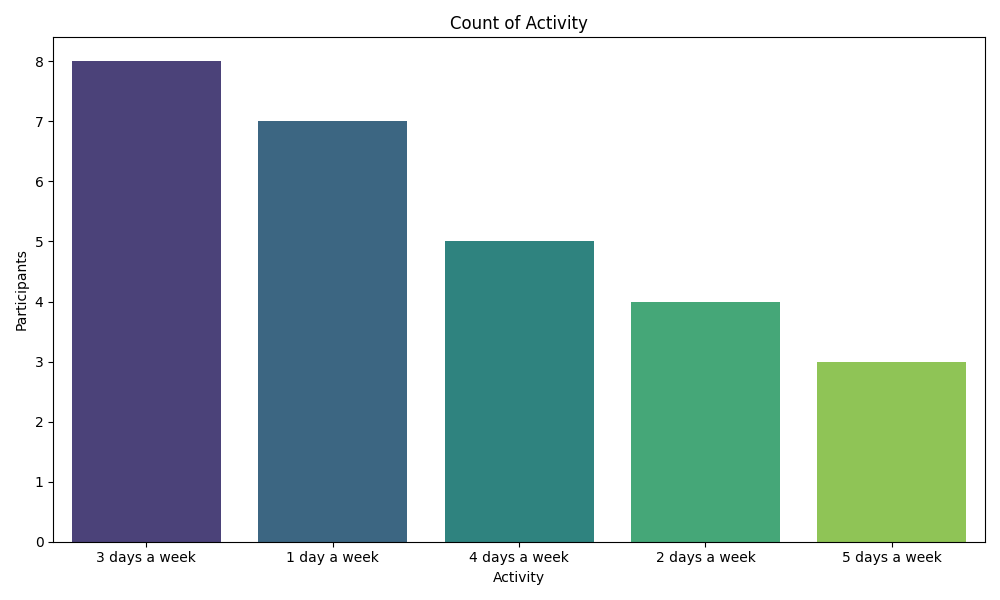
\includegraphics[width=\textwidth]{activity_bar_chart.png}
        \caption{Average use of the building for various activities}
        \label{fig:image1}
    \end{subfigure}
    \hfill
    \begin{subfigure}{0.4\textwidth}
        \centering
        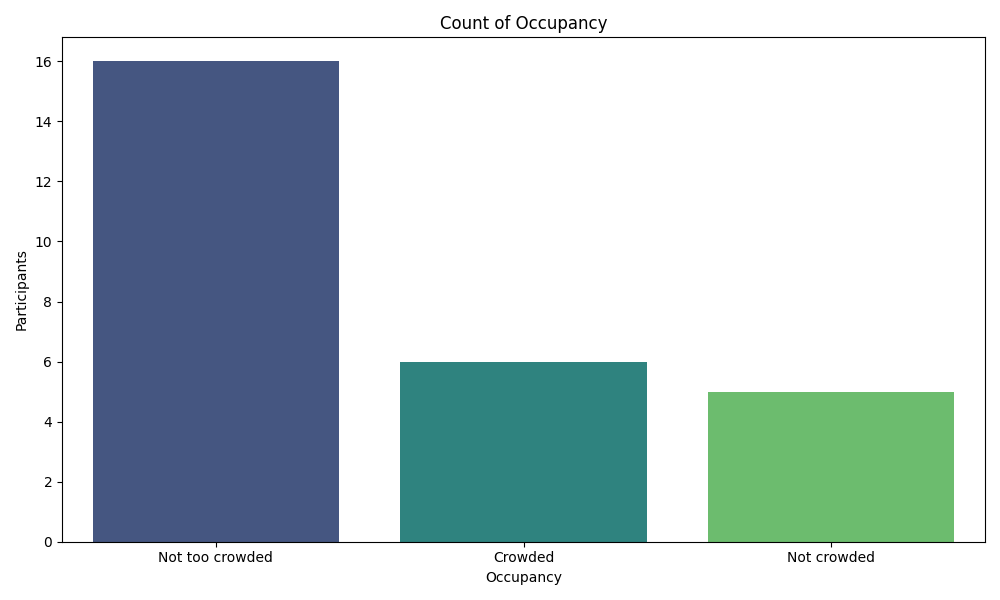
\includegraphics[width=\textwidth]{occupancy_bar_chart.png}
        \caption{Description of occupancy crowdedness}
        \label{fig:image2}
    \end{subfigure}
    \begin{subfigure}{0.4\textwidth}
        \centering
        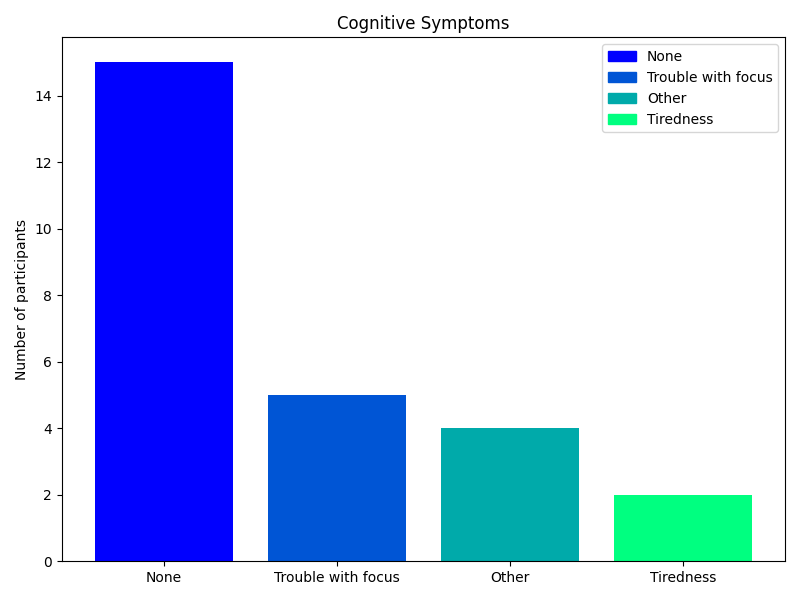
\includegraphics[width=\textwidth]{cognitive_symptomps.png}
        \caption{Cognitive symptons based on the air quality}
        \label{fig:image1}
    \end{subfigure}
    \hfill
    \begin{subfigure}{0.4\textwidth}
        \centering
        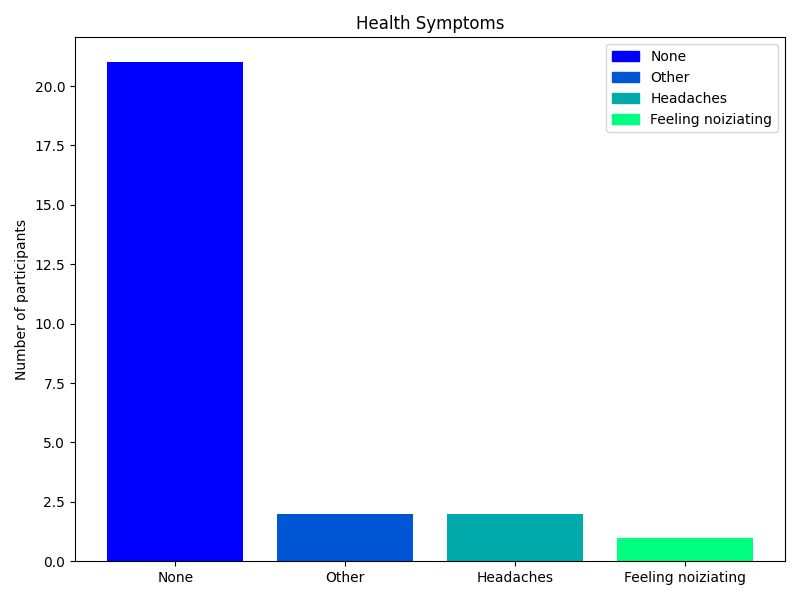
\includegraphics[width=\textwidth]{health_symptomps.png}
        \caption{Health symptons based on the air quality}
        \label{fig:image2}
    \end{subfigure}    
    \caption{Bar charts of the survey questions about activity, occupancy, health and cognitive symptons}
    \label{fig:grid}
\end{figure}

\begin{figure}[htbp]
    \centering
    \begin{subfigure}{0.18\textwidth}
        \centering
        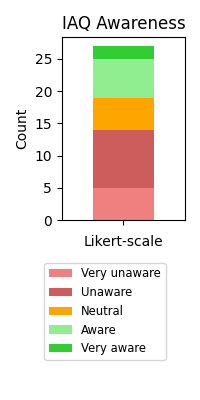
\includegraphics[width=\textwidth]{iaq_awareness.png}
        \caption{Awaneress}
        \label{fig:image1}
    \end{subfigure}
    \hfill
    \begin{subfigure}{0.18\textwidth}
        \centering
        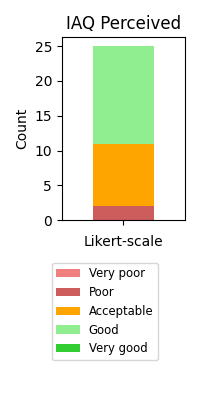
\includegraphics[width=\textwidth]{iaq_perceived.png}
        \caption{Perceived}
        \label{fig:image2}
    \end{subfigure}
    \hfill
    \begin{subfigure}{0.18\textwidth}
        \centering
        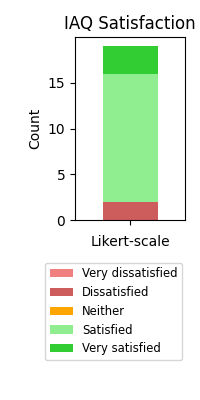
\includegraphics[width=\textwidth]{iaq_satisfaction.png}
        \caption{Satisfaction}
        \label{fig:image2}
    \end{subfigure}    
    \caption{Stacked bar charts of the Likert-scales on IAQ awareness, perceived and satisfaction}
    \label{fig:grid}
\end{figure}

\newpage

\section{Monitor data}
\label{appendix:monitor-data}

\begin{figure}[htbp]
    \centering
    \begin{subfigure}{0.48\textwidth}
        \centering
        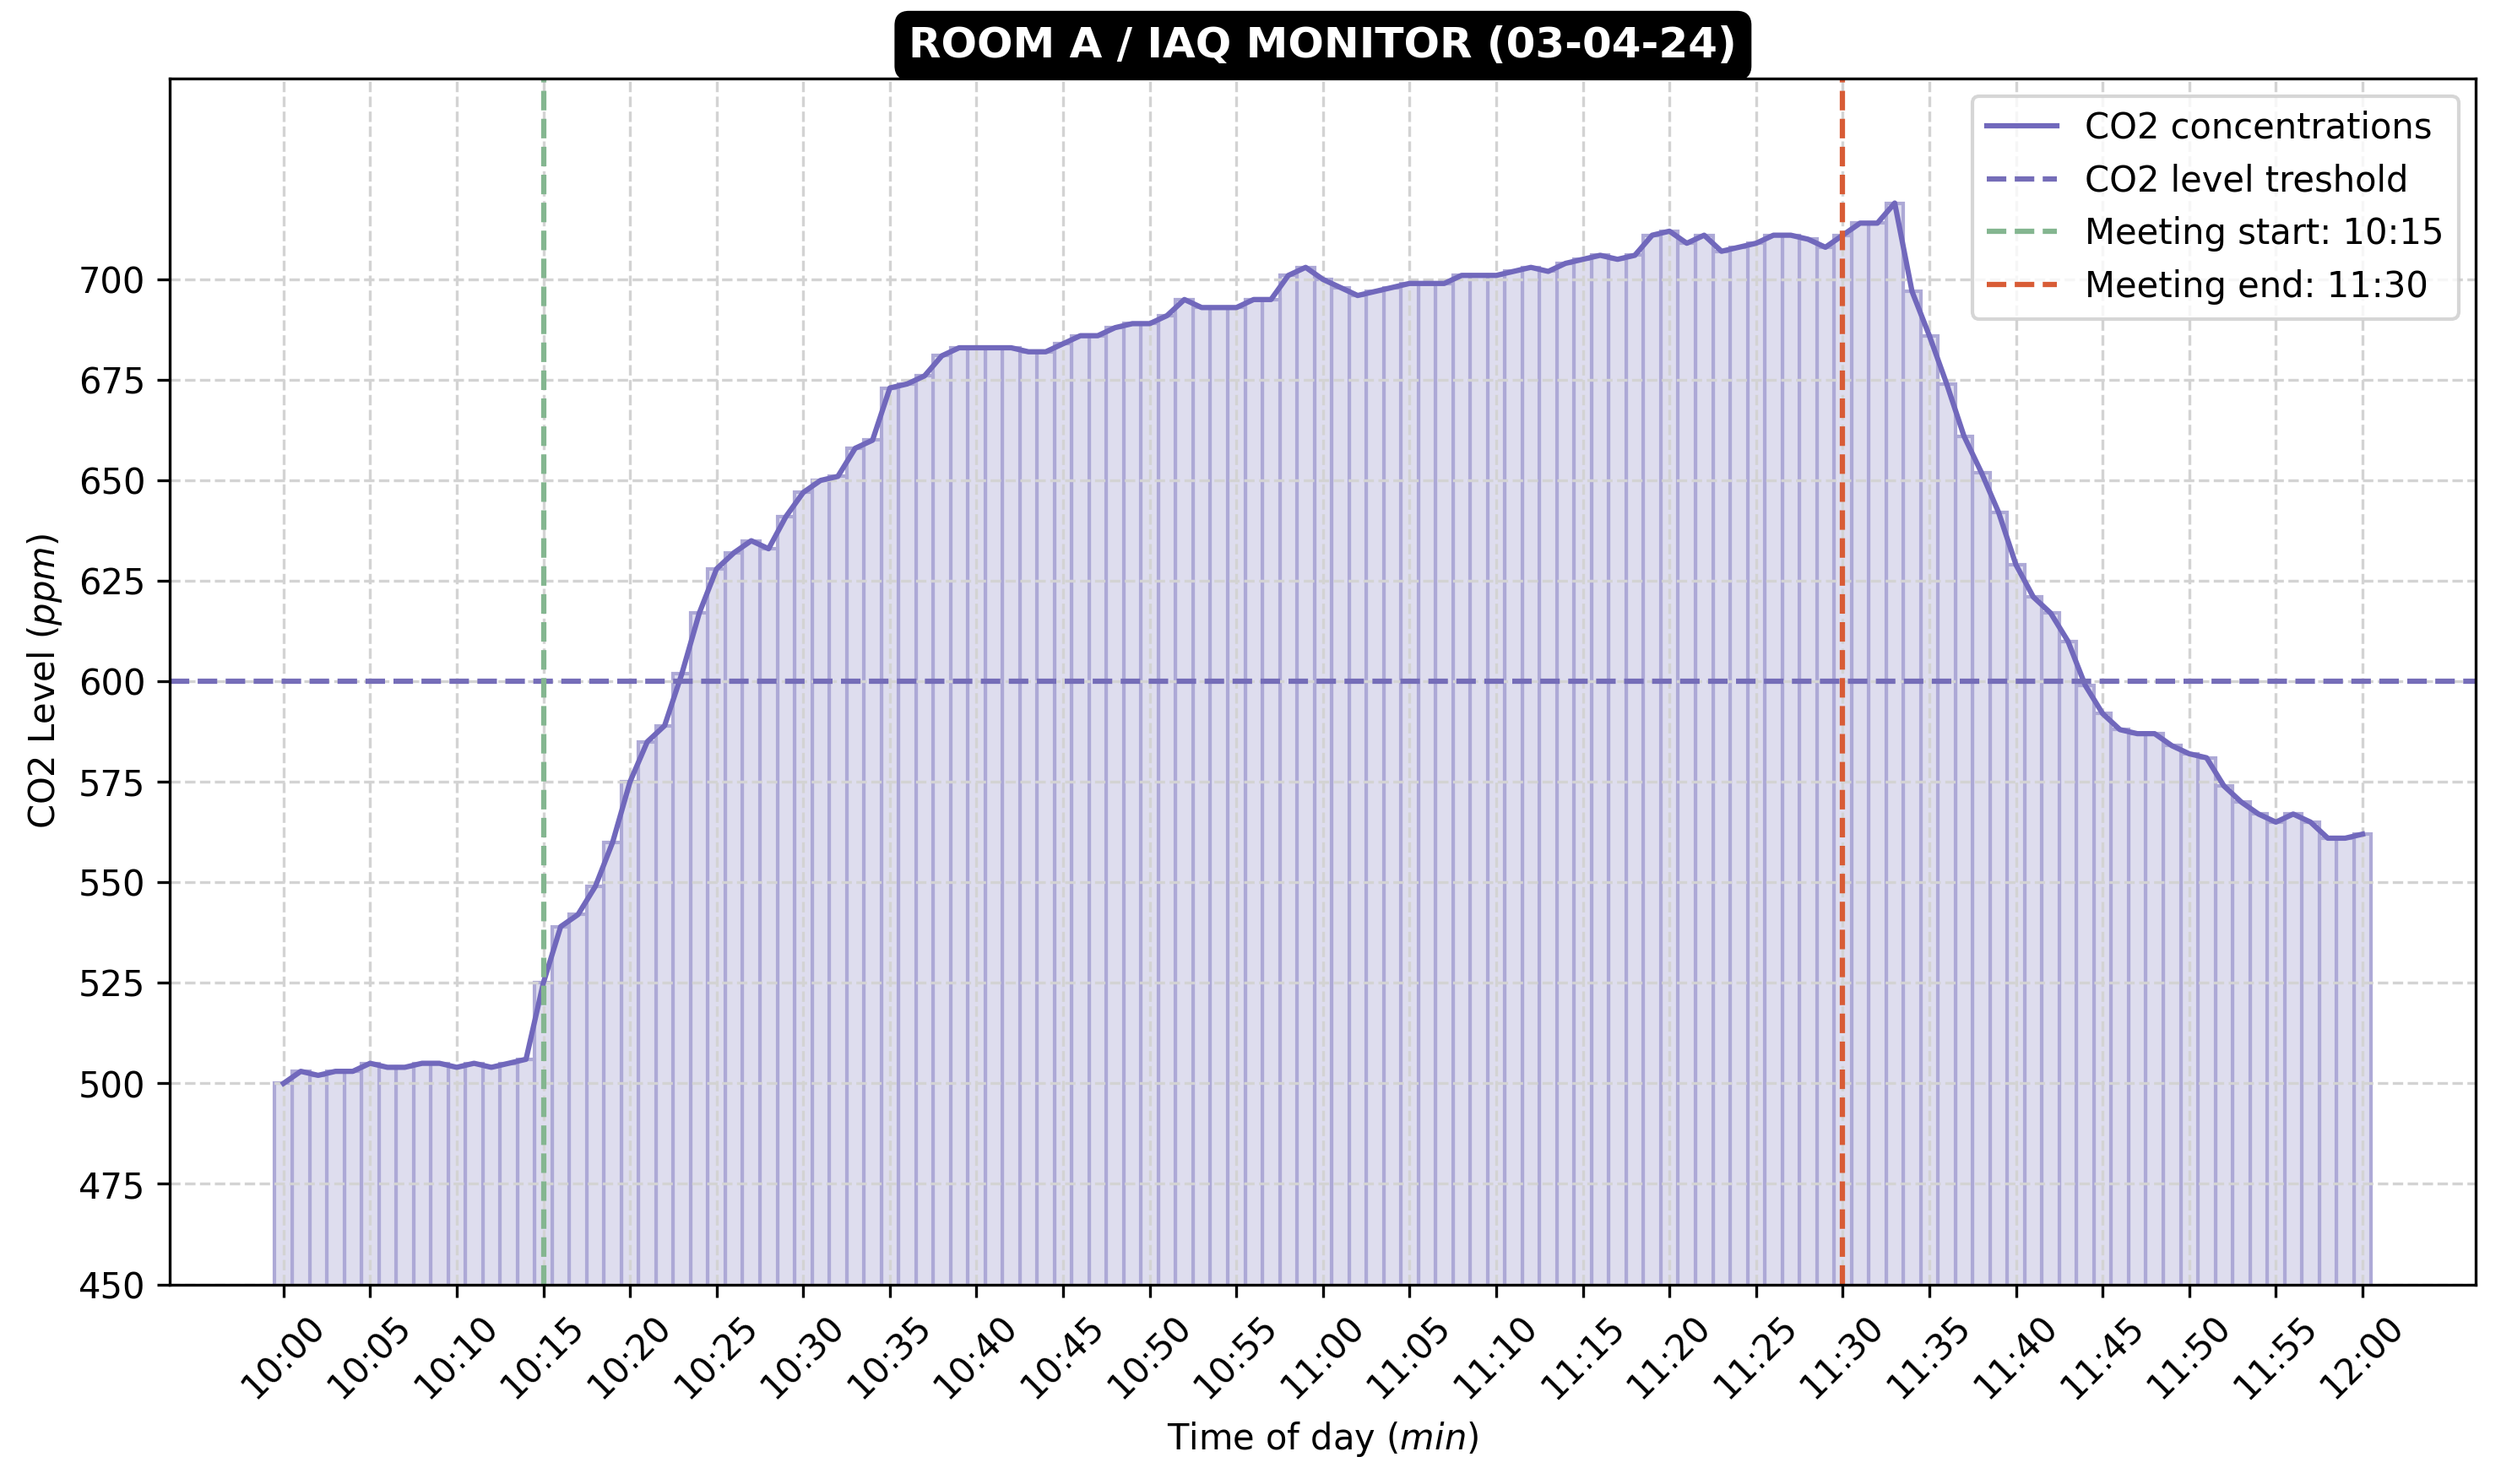
\includegraphics[width=\textwidth]{room-a-monitor-meeting-spike-single.png}
        \caption{Single meeting CO2 concentrations in Room A}
        \label{fig:image1}
    \end{subfigure}
    \hfill
    \begin{subfigure}{0.48\textwidth}
        \centering
        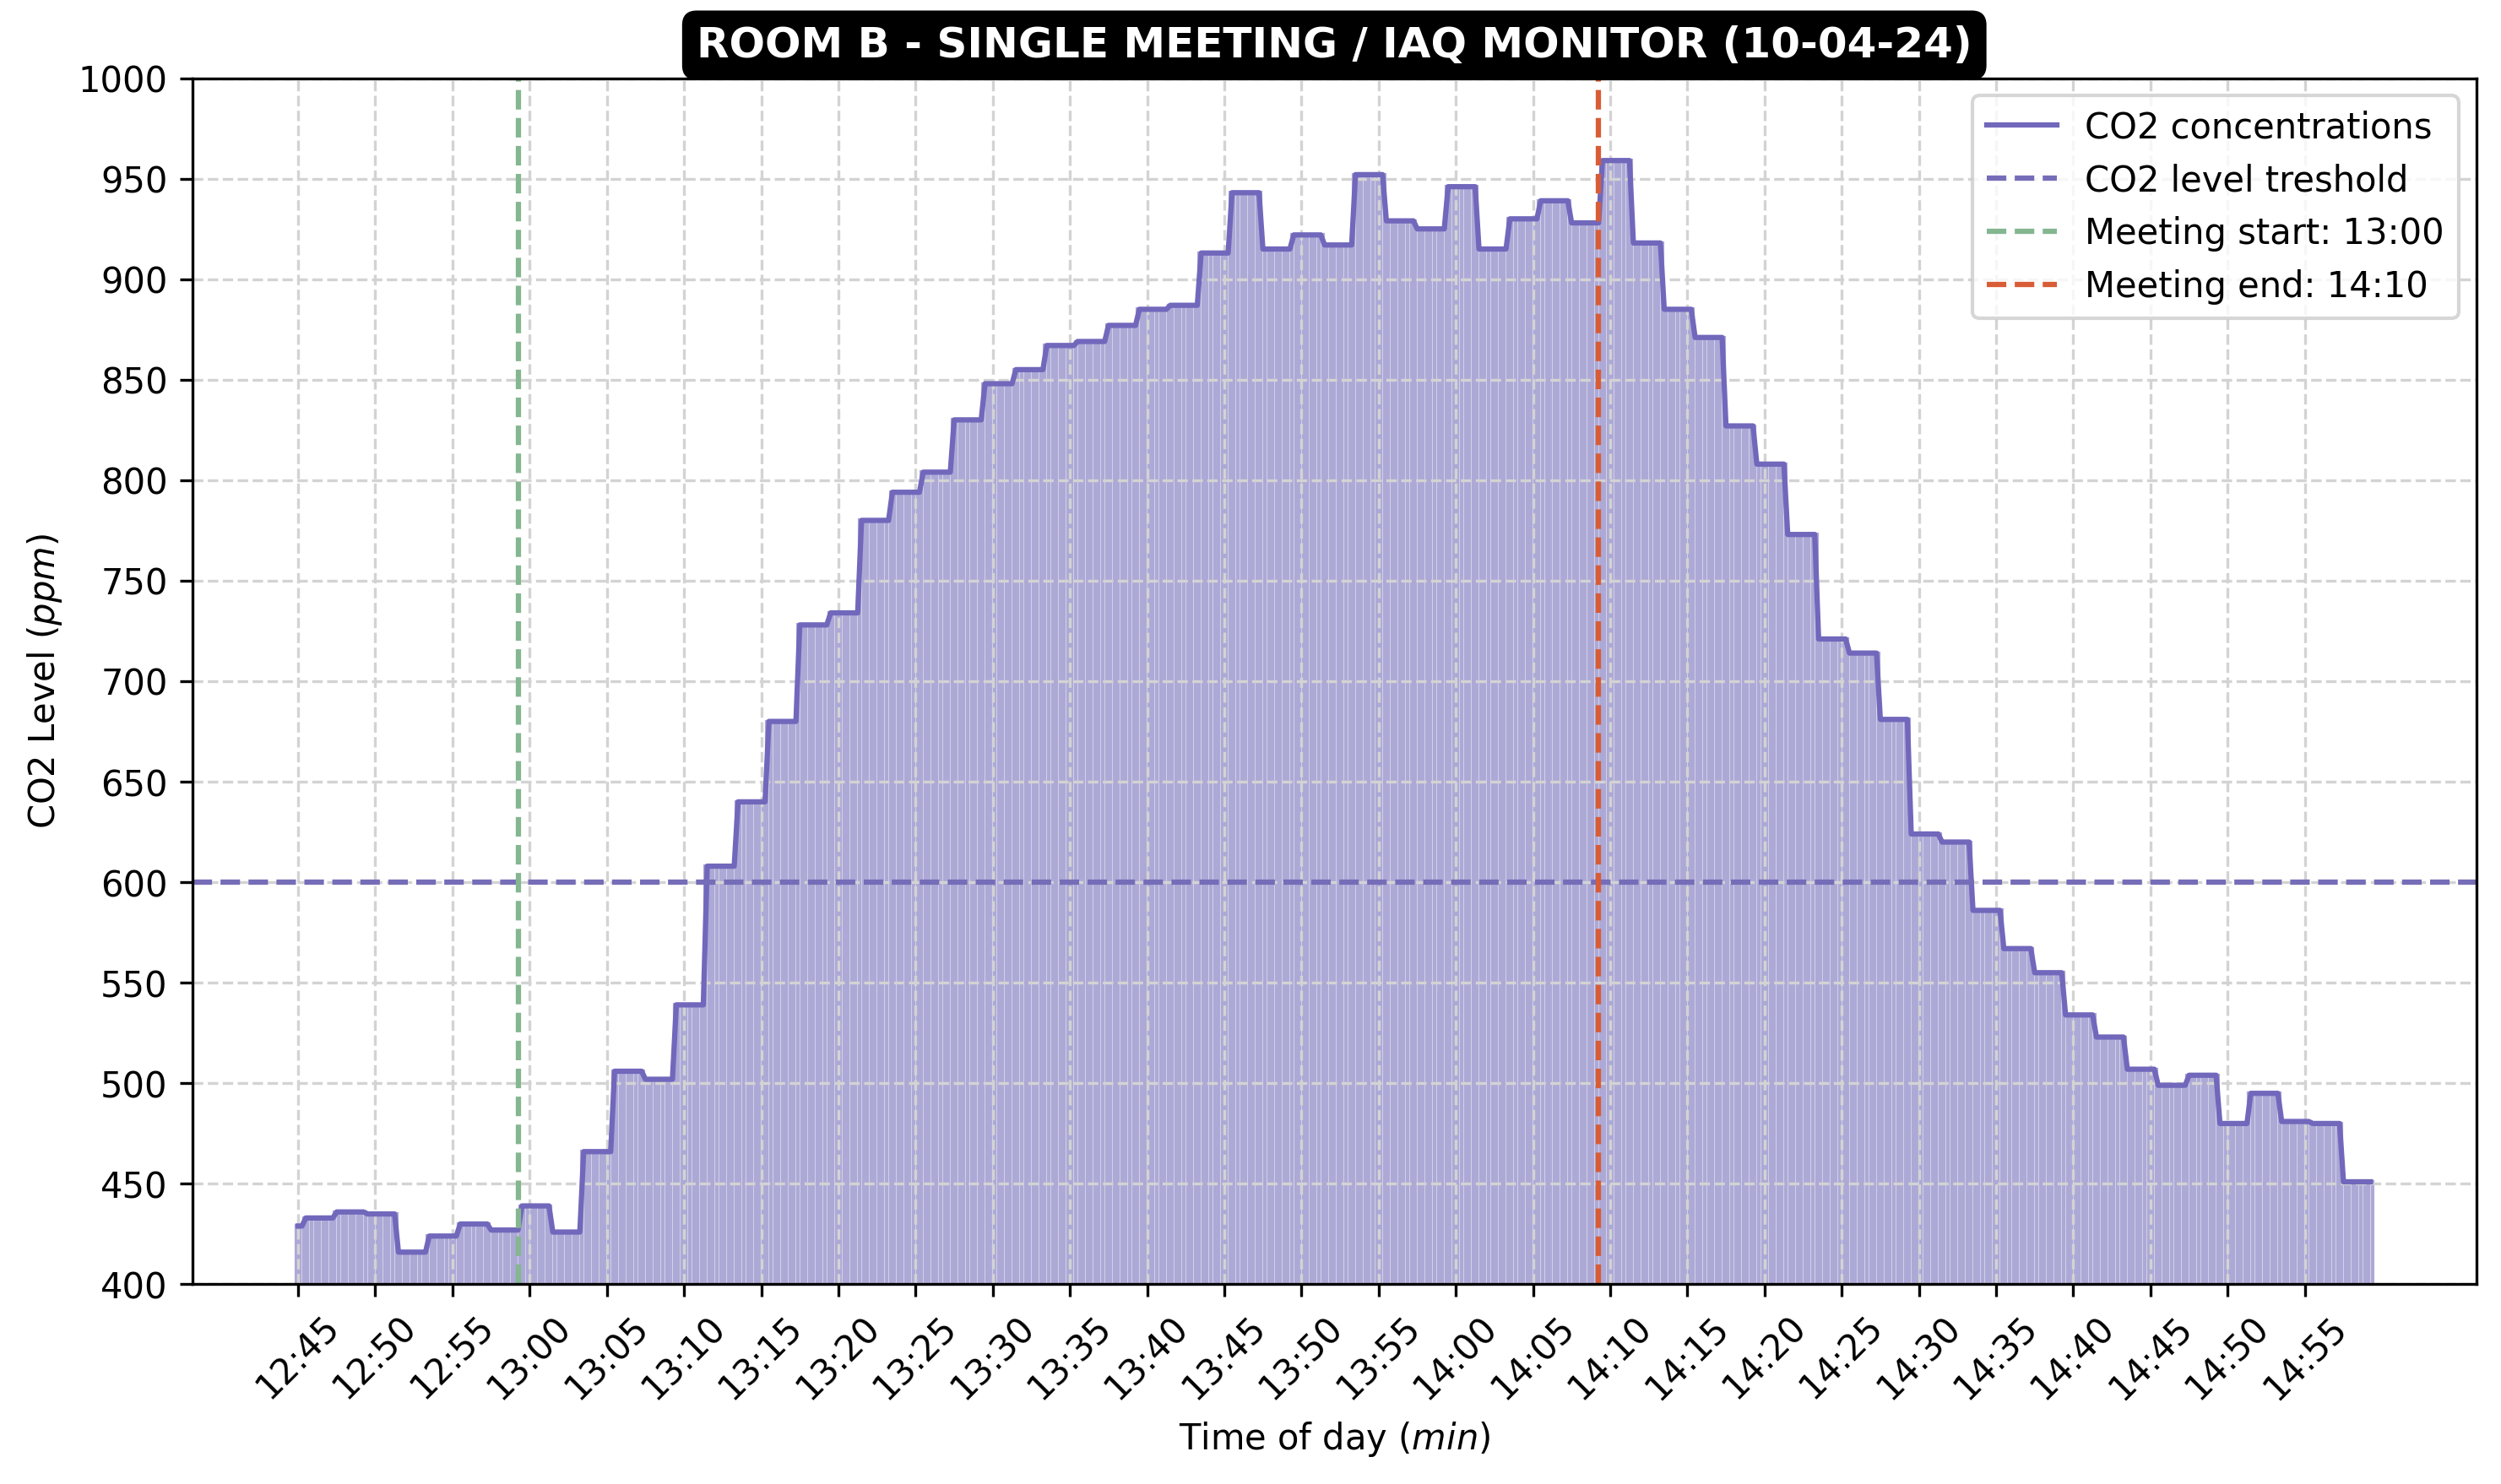
\includegraphics[width=\textwidth]{room-b-monitor-meeting-spike-single.png}
        \caption{Single meeting CO2 concentrations in Room B}
        \label{fig:image2}
    \end{subfigure}
    \caption{IAQ monitoring CO2 concentrations of a single sample meeting based on the start and end time of the meeting}
    \label{fig:grid}
\end{figure}

\begin{figure}[htbp]
    \centering
    \begin{subfigure}{0.48\textwidth}
        \centering
        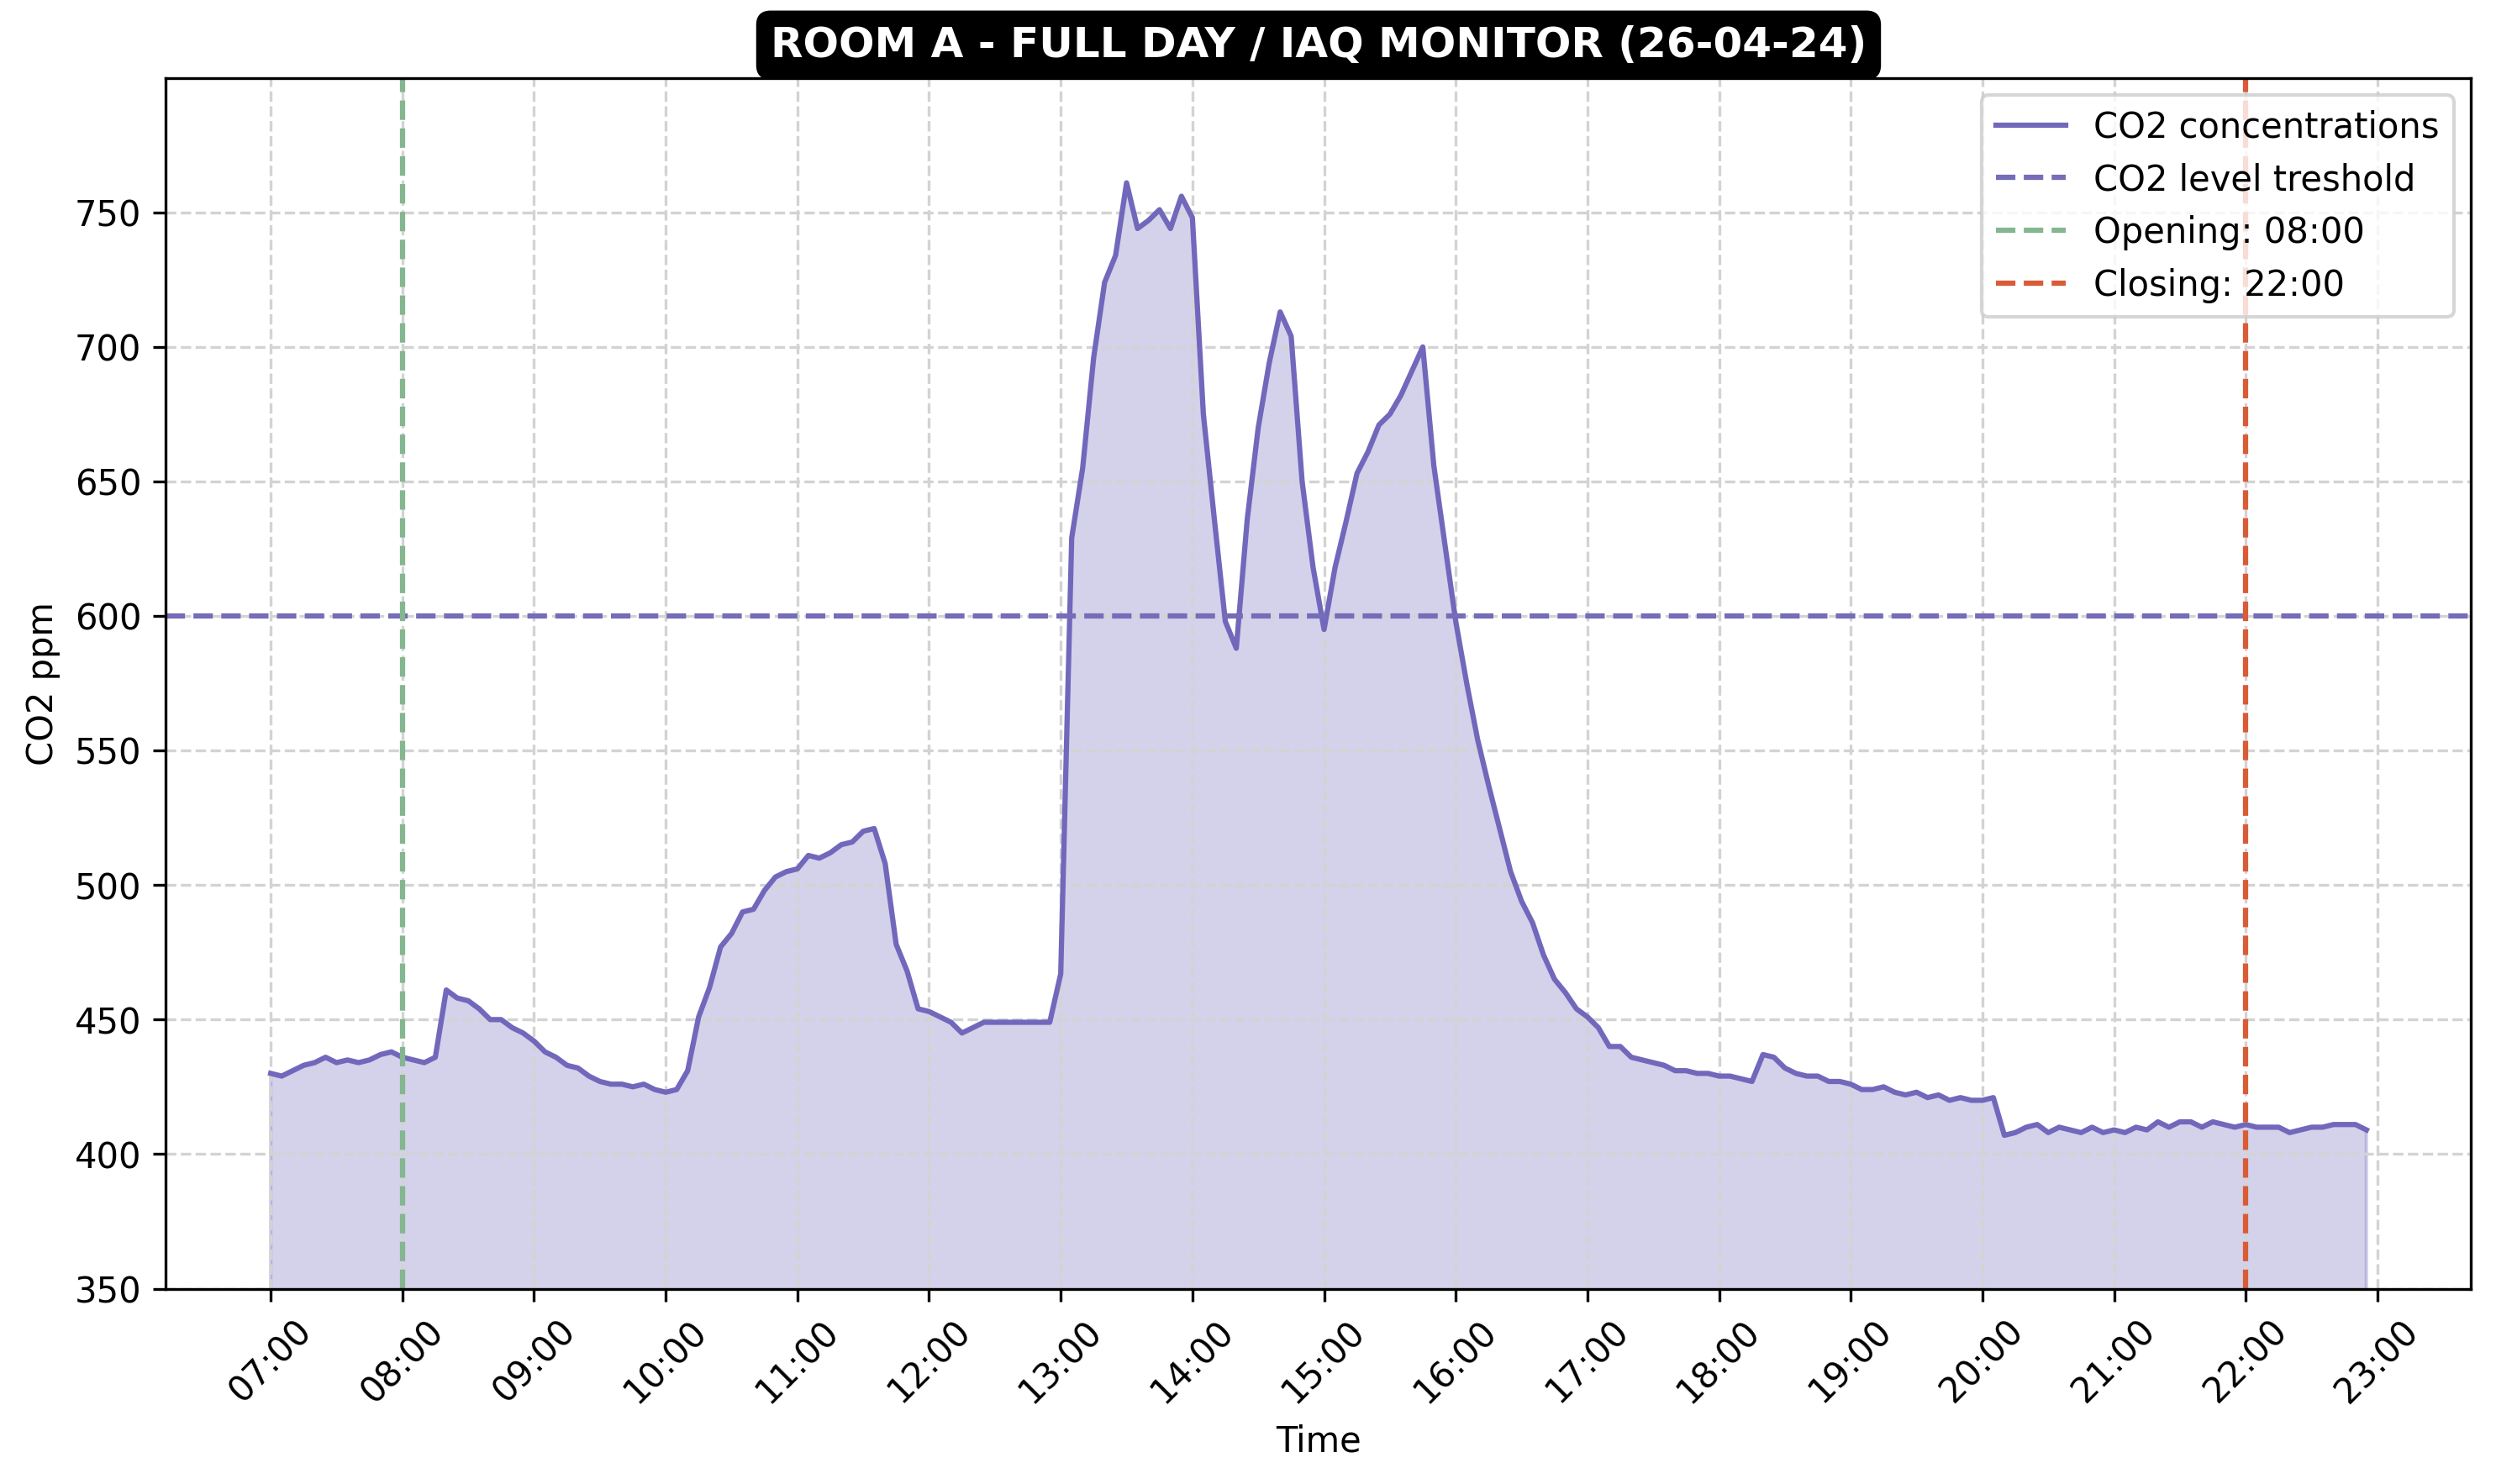
\includegraphics[width=\textwidth]{room-a-monitor-meeting-spike-day.png}
        \caption{A day of meetings CO2 concentrations in Room A}
        \label{fig:image1}
    \end{subfigure}
    \hfill
    \begin{subfigure}{0.48\textwidth}
        \centering
        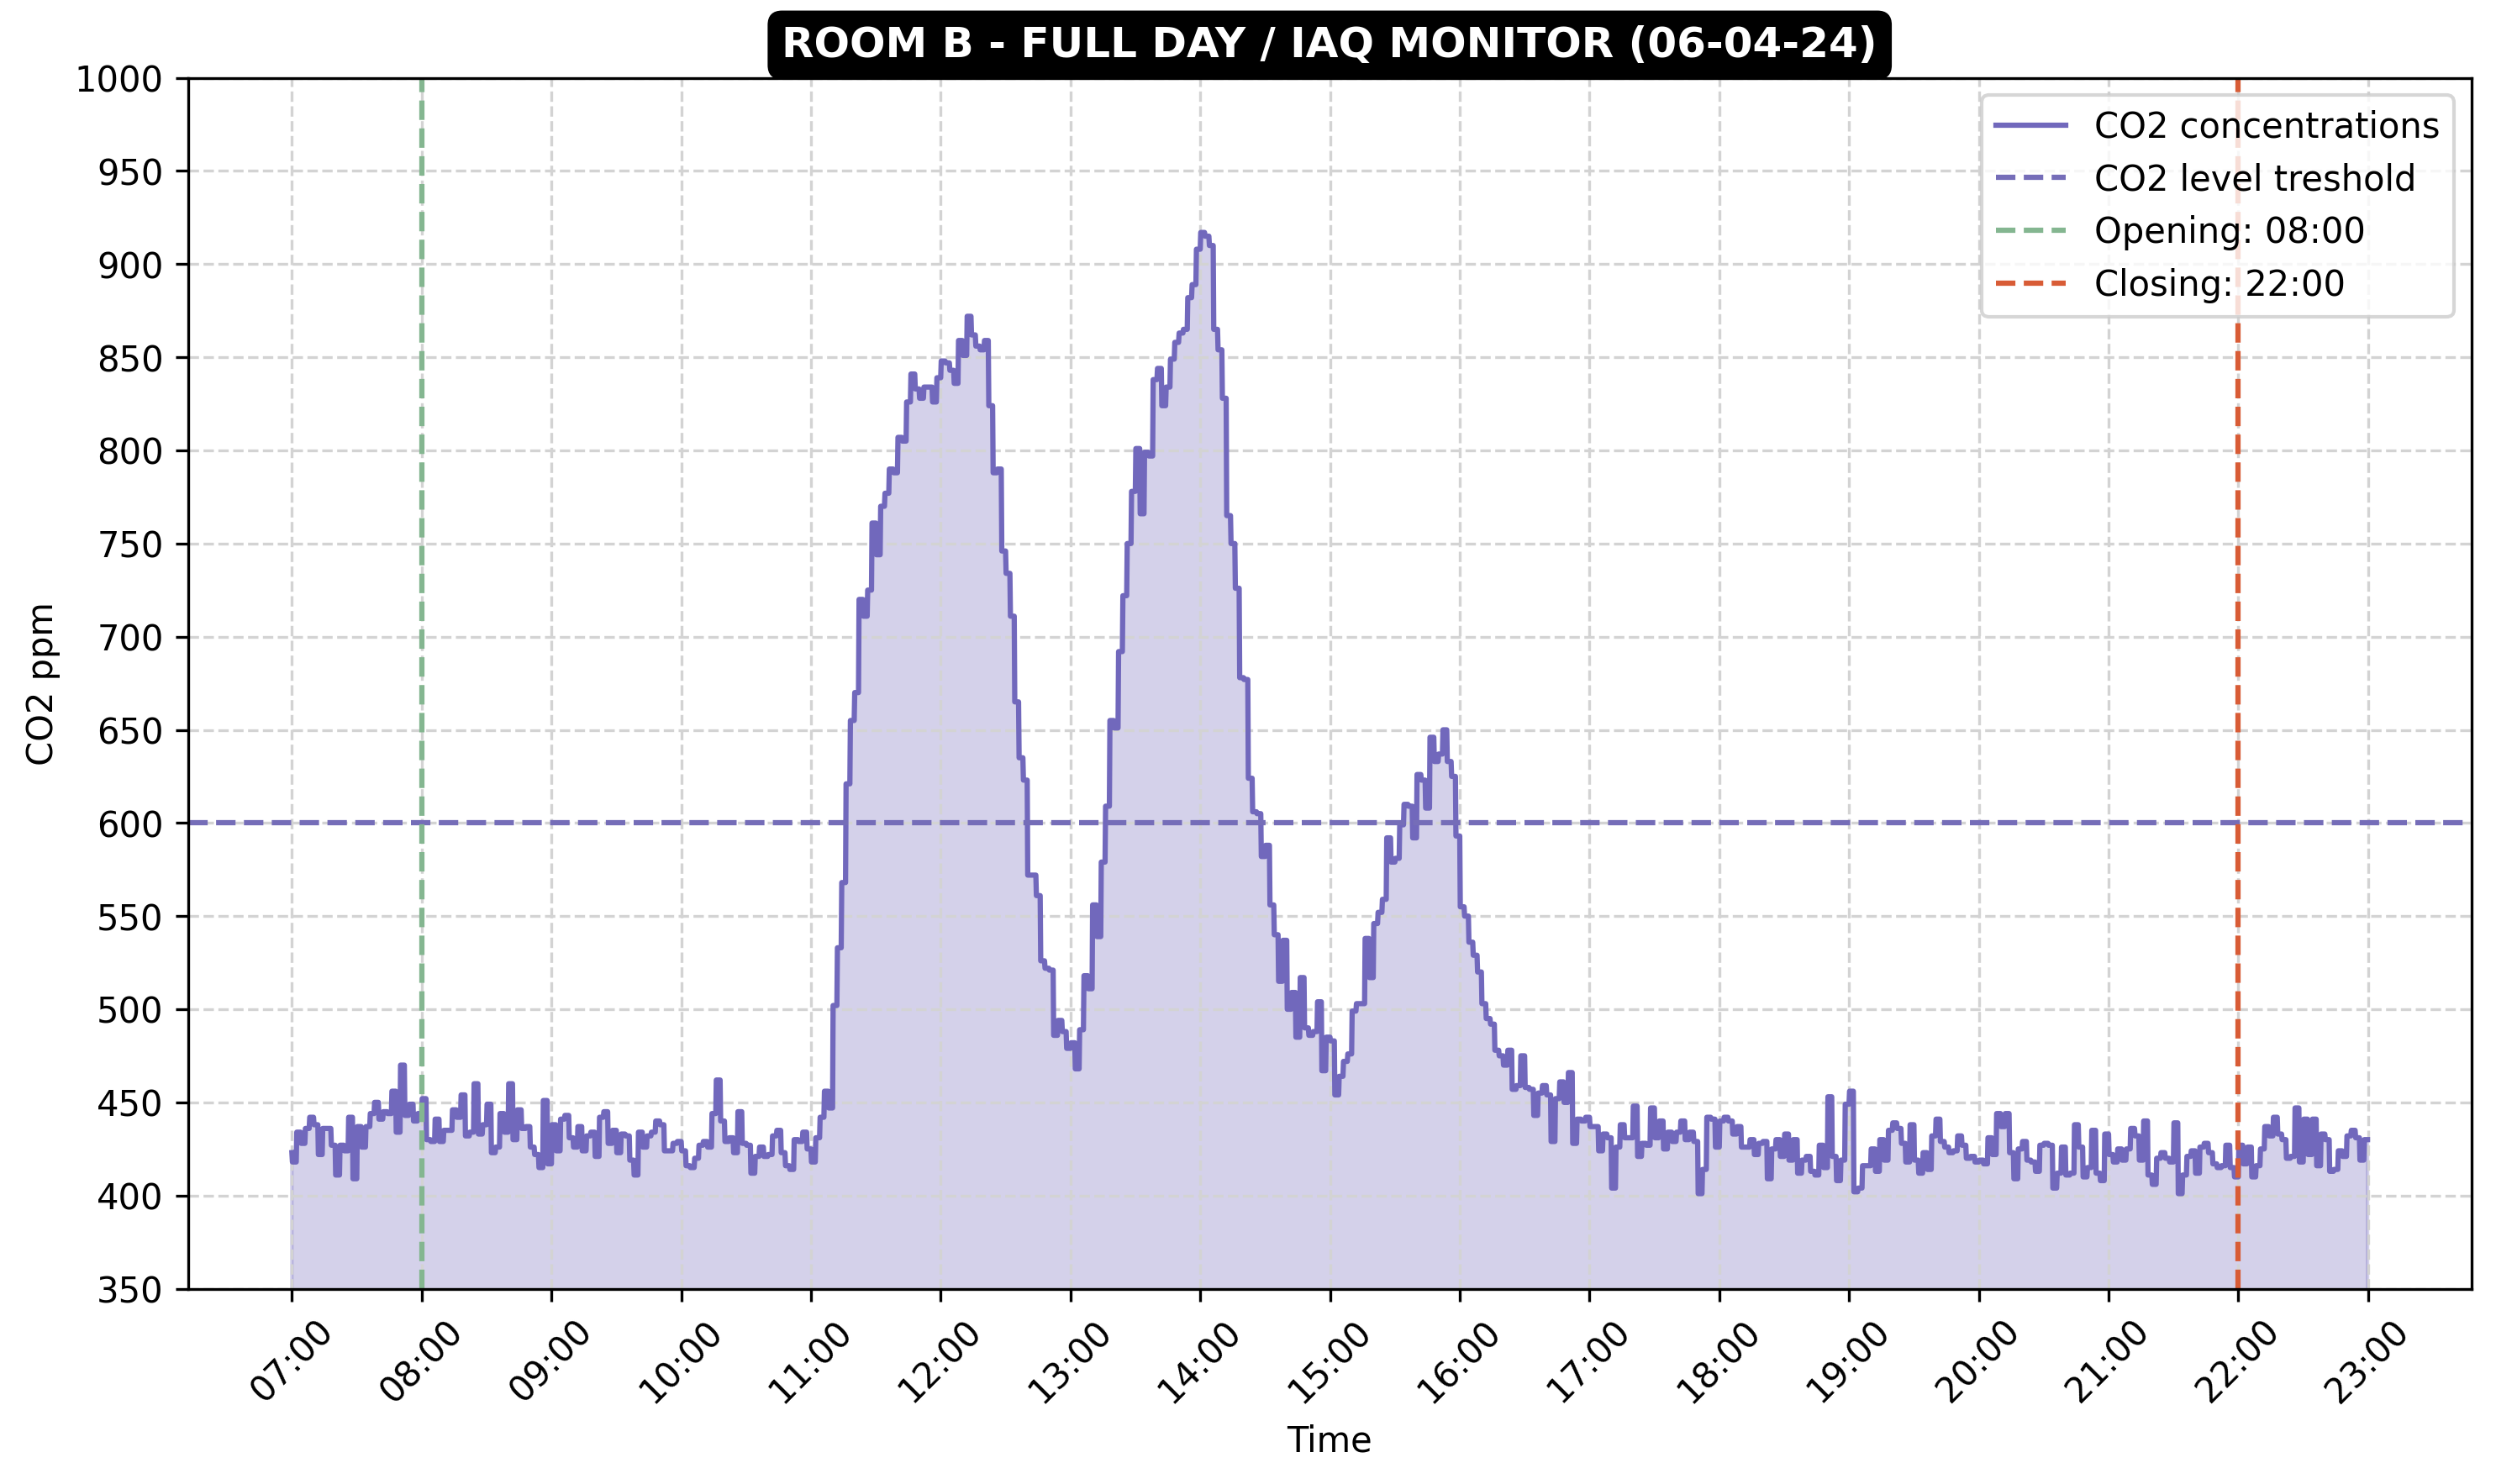
\includegraphics[width=\textwidth]{room-b-monitor-meeting-spike-day.png}
        \caption{A day of meetings CO2 concentrations in Room B}
        \label{fig:image2}
    \end{subfigure}
    \caption{IAQ monitoring CO2 concentrations of a sample day meeting based on the opening hours of the building}
    \label{fig:grid}
\end{figure}

\begin{figure}[htbp]
    \centering
    \begin{subfigure}{0.48\textwidth}
        \centering
        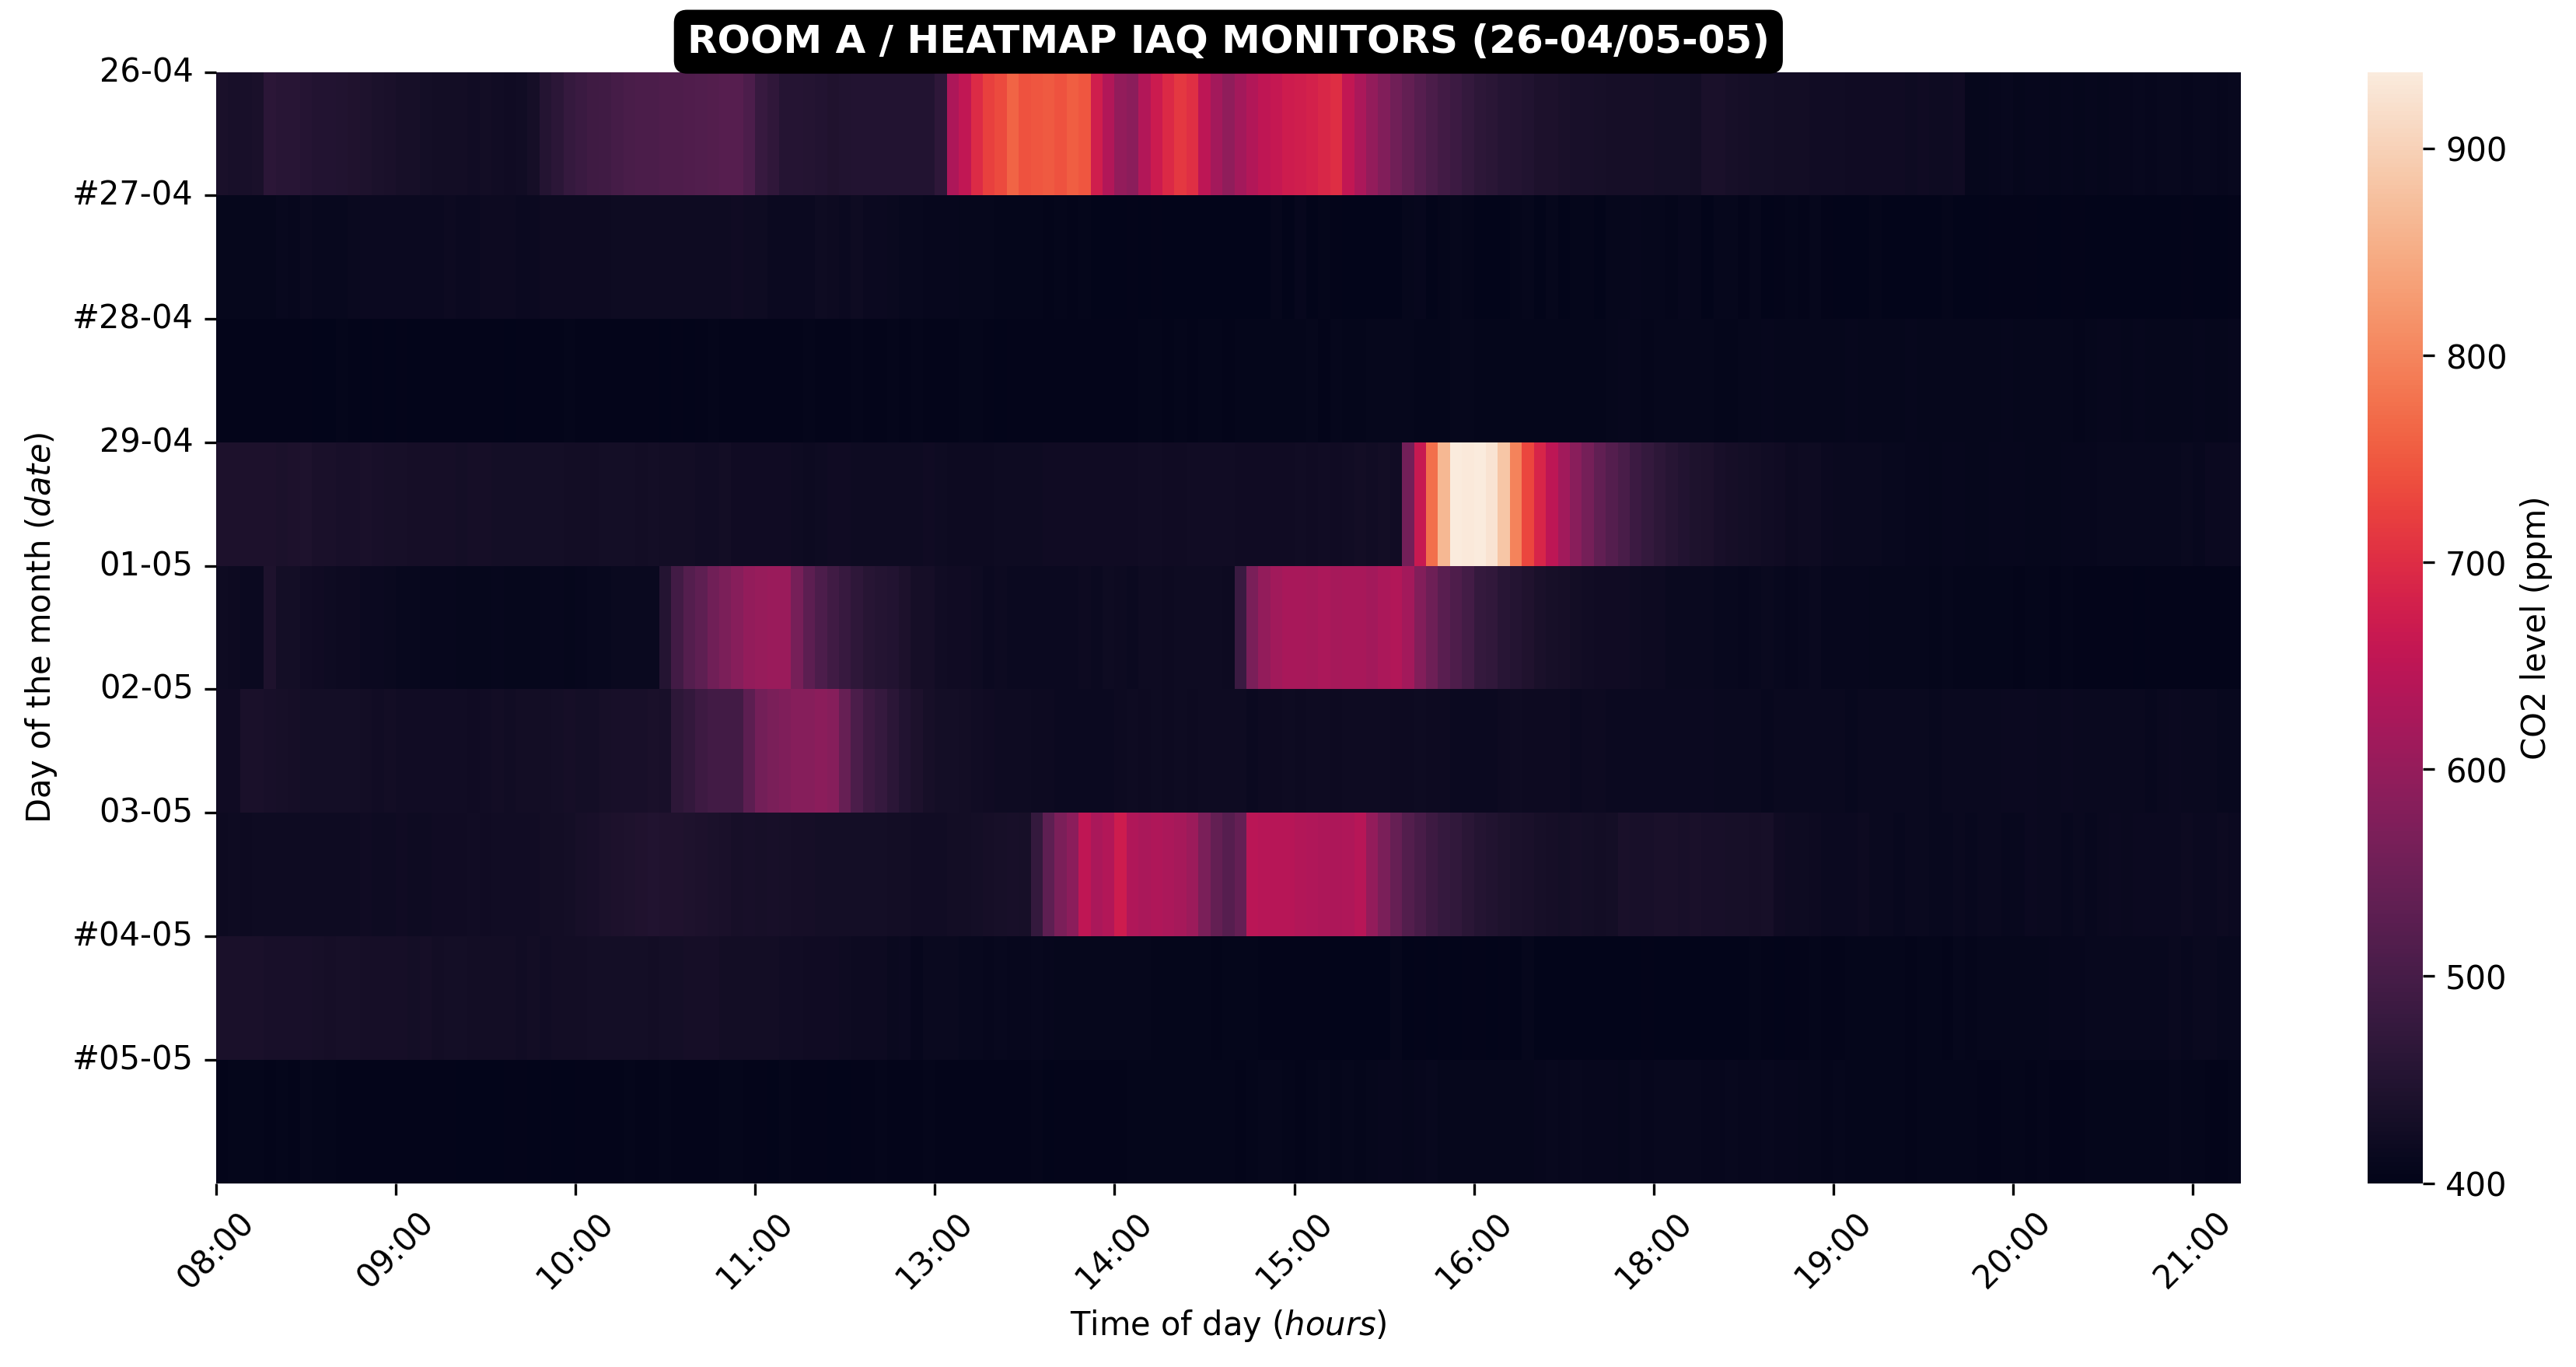
\includegraphics[width=\textwidth]{room-a-monitor-heatmap.png}
        \caption{Heatmap of ten days of monitoring in Room A}
        \label{fig:image1}
    \end{subfigure}
    \hfill
    \begin{subfigure}{0.48\textwidth}
        \centering
        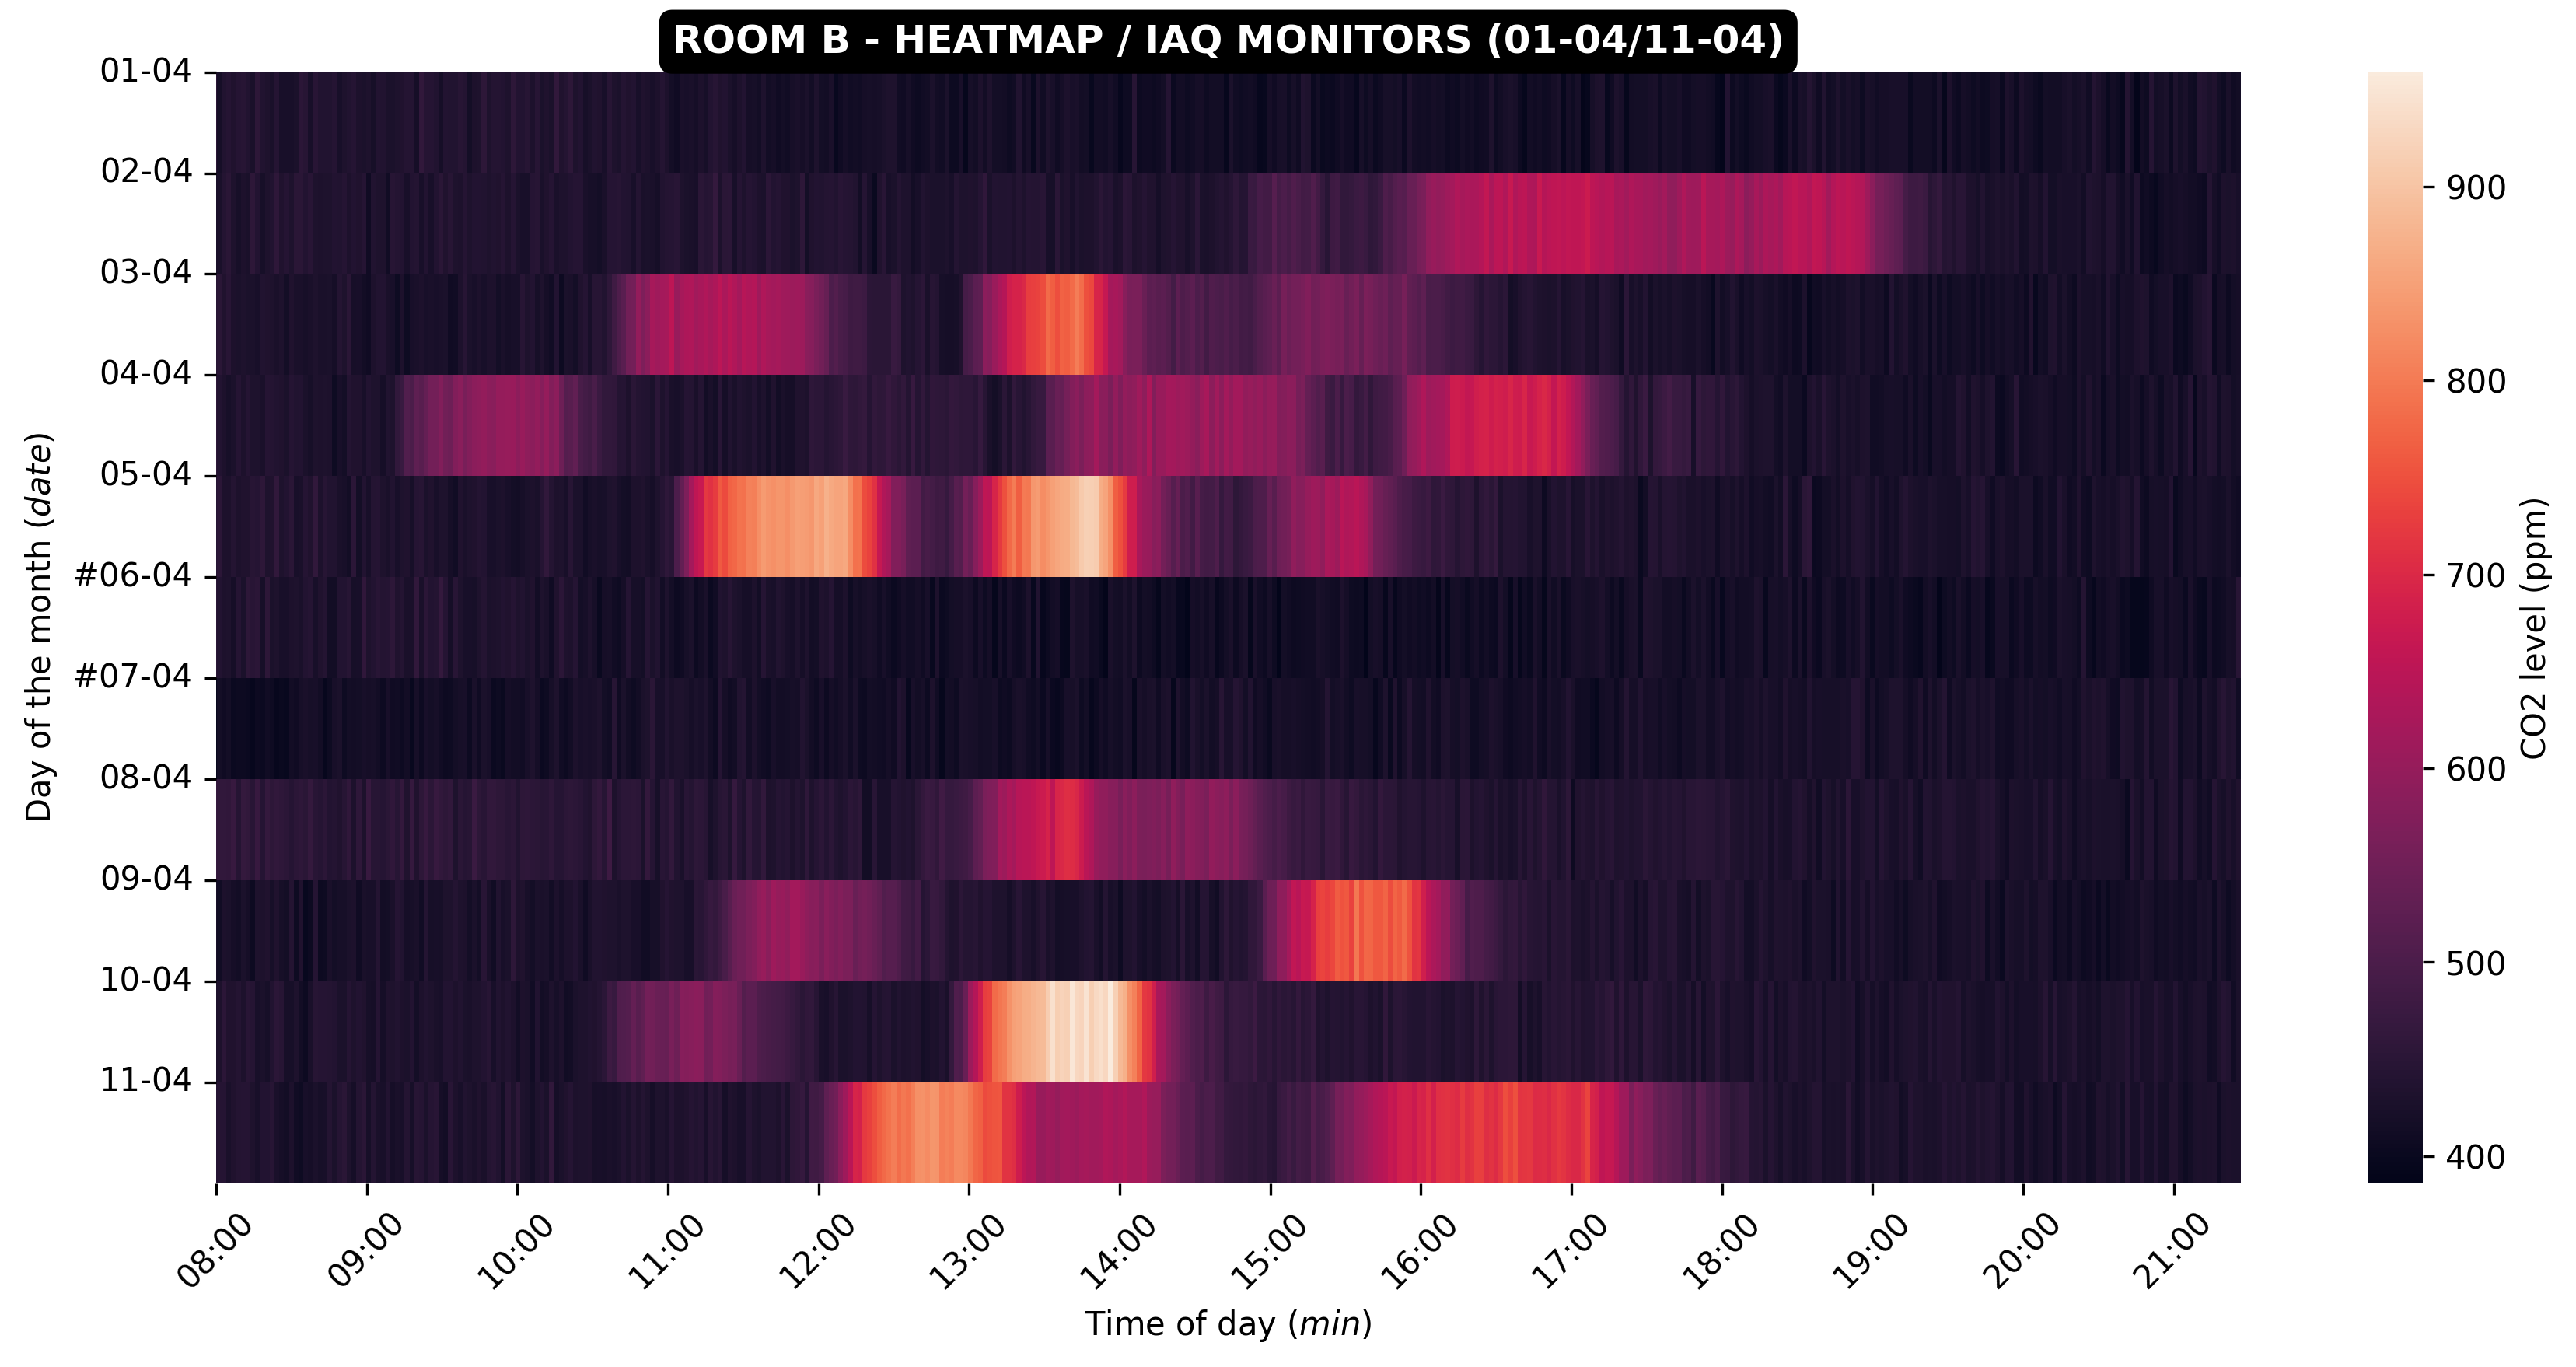
\includegraphics[width=\textwidth]{room-b-monitor-heatmap.png}
        \caption{Heatmap of ten days of monitoring in Room B}
        \label{fig:image2}
    \end{subfigure}
    \caption{IAQ monitoring heatmap CO2 concentrations of the sample ten days based on the opening hours of the building}
    \label{fig:grid}
\end{figure}

\newpage

\section{Evaluation Interviews}
\label{appendix:evaluation}

The evaluation session was conducted in English. The questions and structure below served as a guideline for the interviews. It was a semi-structured interview so the questions acted as guiding questions only. The first part of the evaluation session was done sitting at the meeting room table.

\vspace{5pt}

\textit{\textbf{Introduction:}}

First of all, thank you for participating in this evaluation study researching indoor air quality and testing the proof-of-concept prototype Bluebird. This evaluation study consists of three parts, 1) a semi-structured interview with questions about your activity within this building and notion of IAQ 2) a usability test of the functioning and perception of the prototype and 3) a score questionnaire rating the prototype on several properties. As a participant you cannot do anything wrong, this is a prototype so only it can malfunction. During the testing I will ask you to think out loud and will ocassionaly ask follow-up questions. Pilot tests of this evaluation session indicated that it will take \~50 minutes. \\

\textit{\textbf{Informed Consent:}}

Your participation will be fully anonymized. If you agree, I will record this meeting for archival purposes and transcription. If you feel uncomfortable at any point during this evaluation session, please feel free to stop it at any point. If you don't want to answer any specific questions feel free to state that you would like to skip and I will move on to the next question.

\begin{table}[htbp]
    \captionsetup{justification=raggedright,singlelinecheck=false}
    \caption{\textit{Demographics and role}}
    \label{tab:column_widths}
    \raggedright \textbf{Introduction:} First I'm going to ask some questions about your demographics and use of this building.
    \begin{tabularx}{\textwidth}{|p{0.25\textwidth}|X|}
        \hline
        \textbf{Description} & \textbf{Questions} \\
        \hline
        Demographics for sample size & \textbf{Q1:} What is your age? \\
        & \textbf{Q2:} What gender do you identify with? \\
        & \textbf{Q3:} What is your nationality? \\
        & \textbf{Q4:} What is your level of education? \\
        \hline
        Role of the occupant & 
        \textbf{Q5:} What do you do in daily life for work? \\
        & \textbf{Q6:} How would you describe your role within this building? \\
        & \textbf{Q7:} Where are you usually stationary located in the building? \\
        \hline
    \end{tabularx}
\end{table}

\begin{table}[htbp]
    \captionsetup{justification=raggedright,singlelinecheck=false}
    \caption{\textit{Activity and frequency}}
    \label{tab:column_widths}
    \raggedright \textbf{Introduction:} Now on to some questions about your activity within this building and how you use the meeting rooms.
    \begin{tabularx}{\textwidth}{|p{0.25\textwidth}|X|}
        \hline
        \textbf{Description} & \textbf{Questions} \\
        \hline
        Frequency of activity & \textbf{Q8:} How often do you use this building for various activities? \\
        & \textbf{Q9:} For what types of activities do you usually use the building for? \\
        \hline
        Frequency of meetings & \textbf{Q10:} On average how many meetings do you have per week? \\
        & \textbf{Q11:} On average how long is a typical meeting you attend? \\
        & \textbf{Q12:} What locations do you typically use for your meetings? \\
        \hline
    \end{tabularx}
\end{table}

\begin{table}[htbp]
    \captionsetup{justification=raggedright,singlelinecheck=false}
    \caption{\textit{Notion of Indoor Air Quality (IAQ)}}
    \label{tab:column_widths}
    \raggedright \textbf{Introduction:} Lastly some question about your notion of indoor air quality as a baseline.
    \begin{tabularx}{\textwidth}{|p{0.25\textwidth}|X|}
        \hline
        \textbf{Description} & \textbf{Questions} \\
        \hline
        IAQ awareness & \textbf{Q11:} How aware are you of the current IAQ in this space? 
        \newline
        \textbf{Q12:} How do you perceive the IAQ in this space? \\
        \hline
        Cognitive and health & \textbf{Q13:} Have you ever experienced cognitive symptons related to IAQ in a meeting room? 
        \newline
        \textbf{Q14:} Have you ever experienced health symptons related to IAQ in a meeting room?  \\
        \hline
    \end{tabularx}
\end{table}

\section{Usability tests}
\label{appendix:usability}

For the usability tests we shifted attention towards the prototype that was installed in the meeting room. In all sessions the researcher and occupants stood up and walked towards the prototype. The occupants were allowed to touch the prototype and during the questions the researched changed the state of the prototype so the live movement could be observed.

\vspace{5pt}

\newpage

\textit{\textbf{Introduction:}}

We will move on to testing the prototype. Please imagine you are an occupant having a meeting in the space (meeting room) we are currently in. As you might have noticed on the wall hang from the ceiling, a prototype of a physical artefact is hung up.\\

\begin{table}[htbp]
    \captionsetup{justification=raggedright,singlelinecheck=false}
    \caption{\textit{Understanding of the prototype (learnability)}} 
    \raggedright \textbf{Introduction:} To gather some first impressions I would like to get some description of the prototype based on your view of it.
    \label{tab:column_widths}
    \begin{tabularx}{\textwidth}{|p{0.25\textwidth}|X|}
        \hline
        \textbf{Description} & \textbf{Questions} \\
        \hline
        Description of prototype & \textbf{Q1:} Could you describe in your own words what the physical artefact is? \\
        \hline
        Look and feel & 
        \textbf{Q2:} What do you think of the overall design of the physical artefact? \\
        \hline
        Use of materials & 
        \textbf{Q3:} What do you think of the materials the physical artefact is made of? \\
        \hline
        Communicative properties & 
        \textbf{Q4:} What properties do you think the data physicalization communicates?\\
        \hline        
    \end{tabularx}
\end{table}

\begin{table}[htbp]
    \captionsetup{justification=raggedright,singlelinecheck=false}
    \caption{\textit{Self-reflection (memorability)}}
    \raggedright \textbf{Introduction:} I want to gain insight into how likely you are to take preventitive action based on data insights.
    \label{tab:column_widths}
    \begin{tabularx}{\textwidth}{|p{0.25\textwidth}|X|}
        \hline
        \textbf{Description} & \textbf{Questions} \\
        \hline
        Behavourial change & 
        \textbf{Q5:} How and to what extent do you think your awareness of IAQ changes? \\
        & \textbf{Q6:} How willingly are you to take preventitive action based on the data insights the artefact provides? \\
        \hline
    \end{tabularx}
\end{table}


\begin{table}[htbp]
    \captionsetup{justification=raggedright,singlelinecheck=false}
    \caption{\textit{Design improvements}}
    \raggedright \textbf{Introduction:} After interacting with the prototype for a bit. This usability test concludes with suggestions for design improvements.
    \label{tab:column_widths}
    \begin{tabularx}{\textwidth}{|p{0.25\textwidth}|X|}
        \hline
        \textbf{Description} & \textbf{Questions} \\
        \hline
        Good characteristics & \textbf{Q7:} What are good characteristics of the design of the prototype? \\
        \hline
        Design improvements & \textbf{Q8:} What are shortcomings of the design of the prototype? \\
        \hline
        Further development & \textbf{Q9:} Is there anything that you would wish to be considered further development of the prototype? \\
        \hline
    \end{tabularx}
\end{table}

\section{Effectiveness scores}
\label{appendix:effectiveness}

That concluded the usability test, thank you for thinking out loud and suggesting improvements. The last part is an online score rating statements and hypothesis about the prototype. The occupant and researcher sit down on the table again and the occupant is handed an iPad to fill-in an online questionnaire on Qualtrics with scores.

\vspace{5pt}

\textit{\textbf{Introduction:}}

Lastly, I will give you an online form with statements, in the form of hypothesis. Please rate each of these statements on a score between 1 and 5.\\

\begin{table}[htbp]
    \captionsetup{justification=raggedright,singlelinecheck=false}
    \caption{\textit{Effectiveness scores}}
    \label{tab:column_widths}
    \begin{tabularx}{\textwidth}{|X|X|}
        \hline
        \multicolumn{1}{|p{0.33\textwidth}|}{\textbf{Description}} & \multicolumn{1}{p{0.6\textwidth}|}{\textbf{Statements (Six-point scale)}} \\
        \hline
        Enjoyment & \textbf{S1:} I enjoyed viewing the data physicalization and interacting with the prototype \\
        \hline
        Usefullnes & I derived insights into state of the indoor air quality \\
        \hline
        Effectiveness & I likely will change my behaviour and take preventive measures based on the data insights \\        
    \end{tabularx}
\end{table}

\textit{\textbf{Final remarks:}}

That marks the end of this evaluation session. Thank you so much for your valuable time, insights and feedback. Do you have any other final remarks you want to share about the prototype? \\

\newpage

\section{Concept diagrams}
\label{appendix:conceptdiagrams}

Design diagrams of the brainstormed concepts in medium-fi sketches that show the component breakdown and interaction states.

\begin{figure}[H]
    \centering
    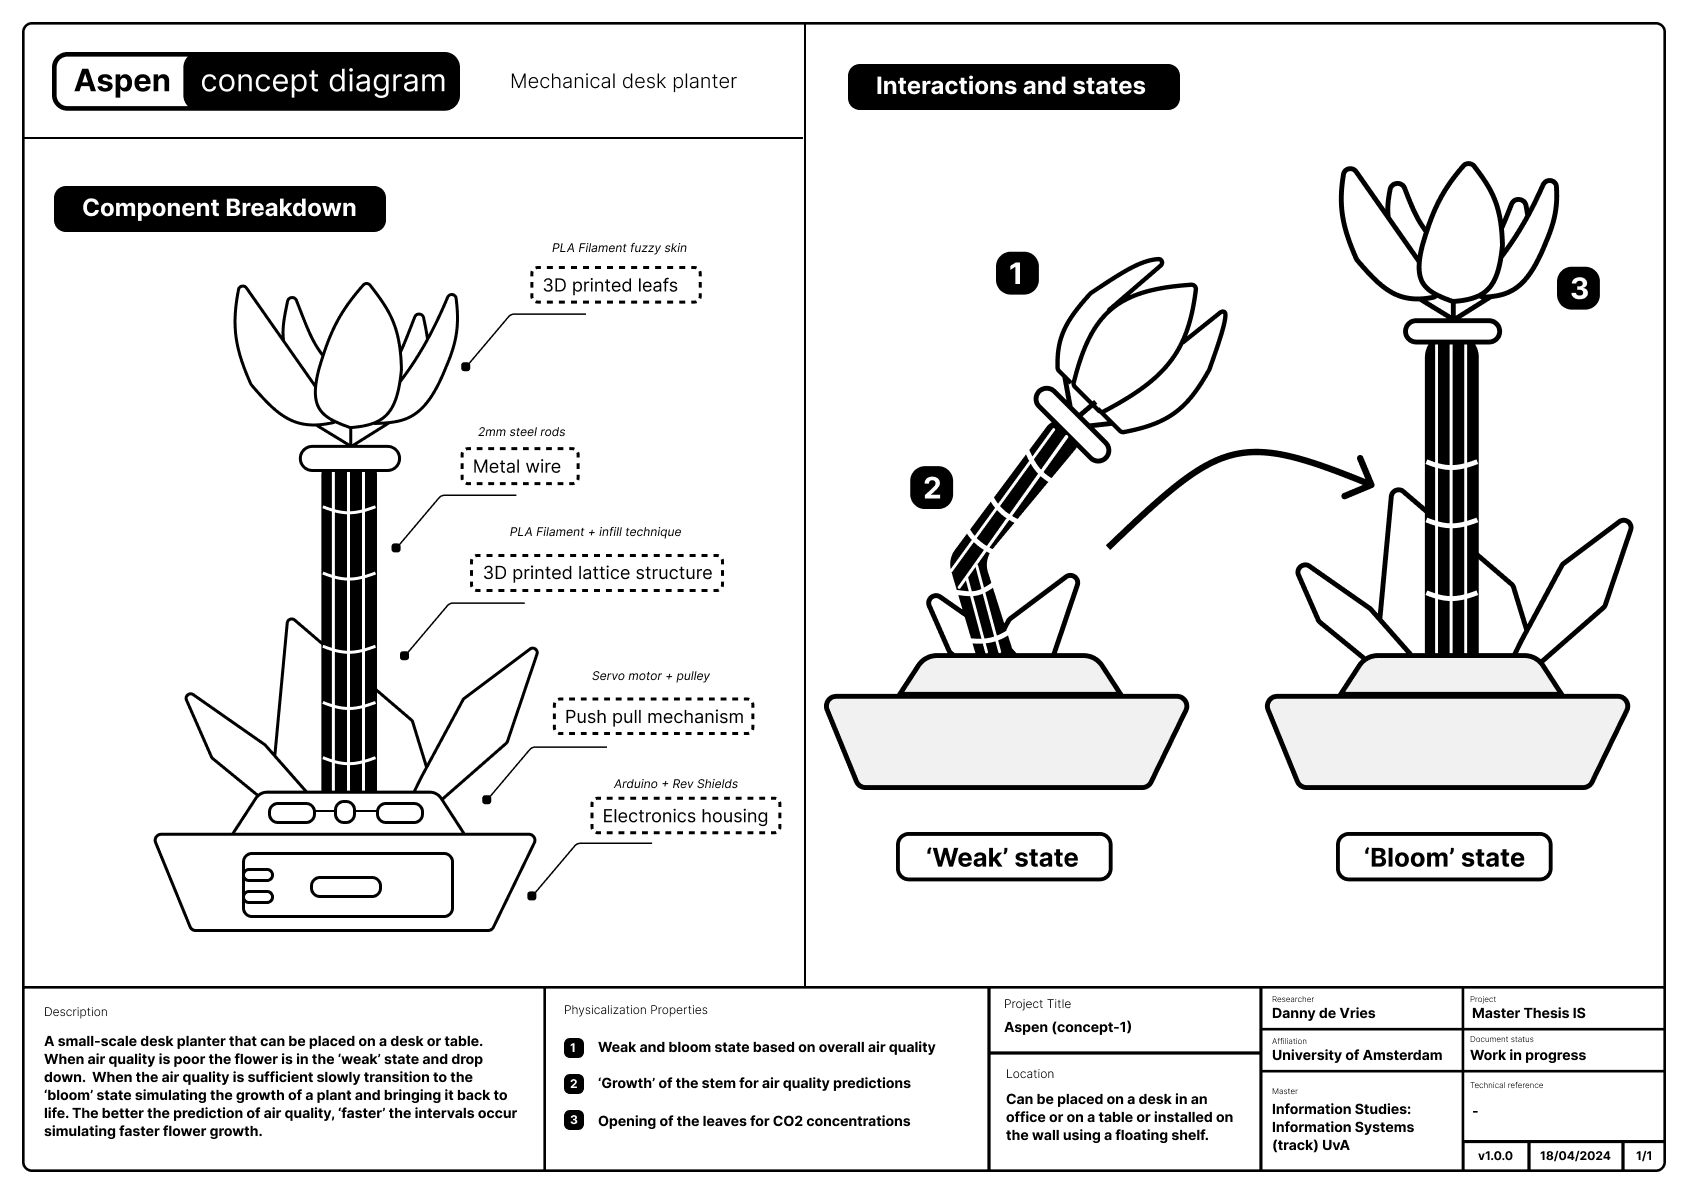
\includegraphics[width=0.6\paperwidth]{Concept-1_Aspen_Design_Diagram.jpg}
    \caption{Design diagram of Concept-2}
    \label{fig:timeline}
\end{figure}

\begin{figure}[H]
    \centering
    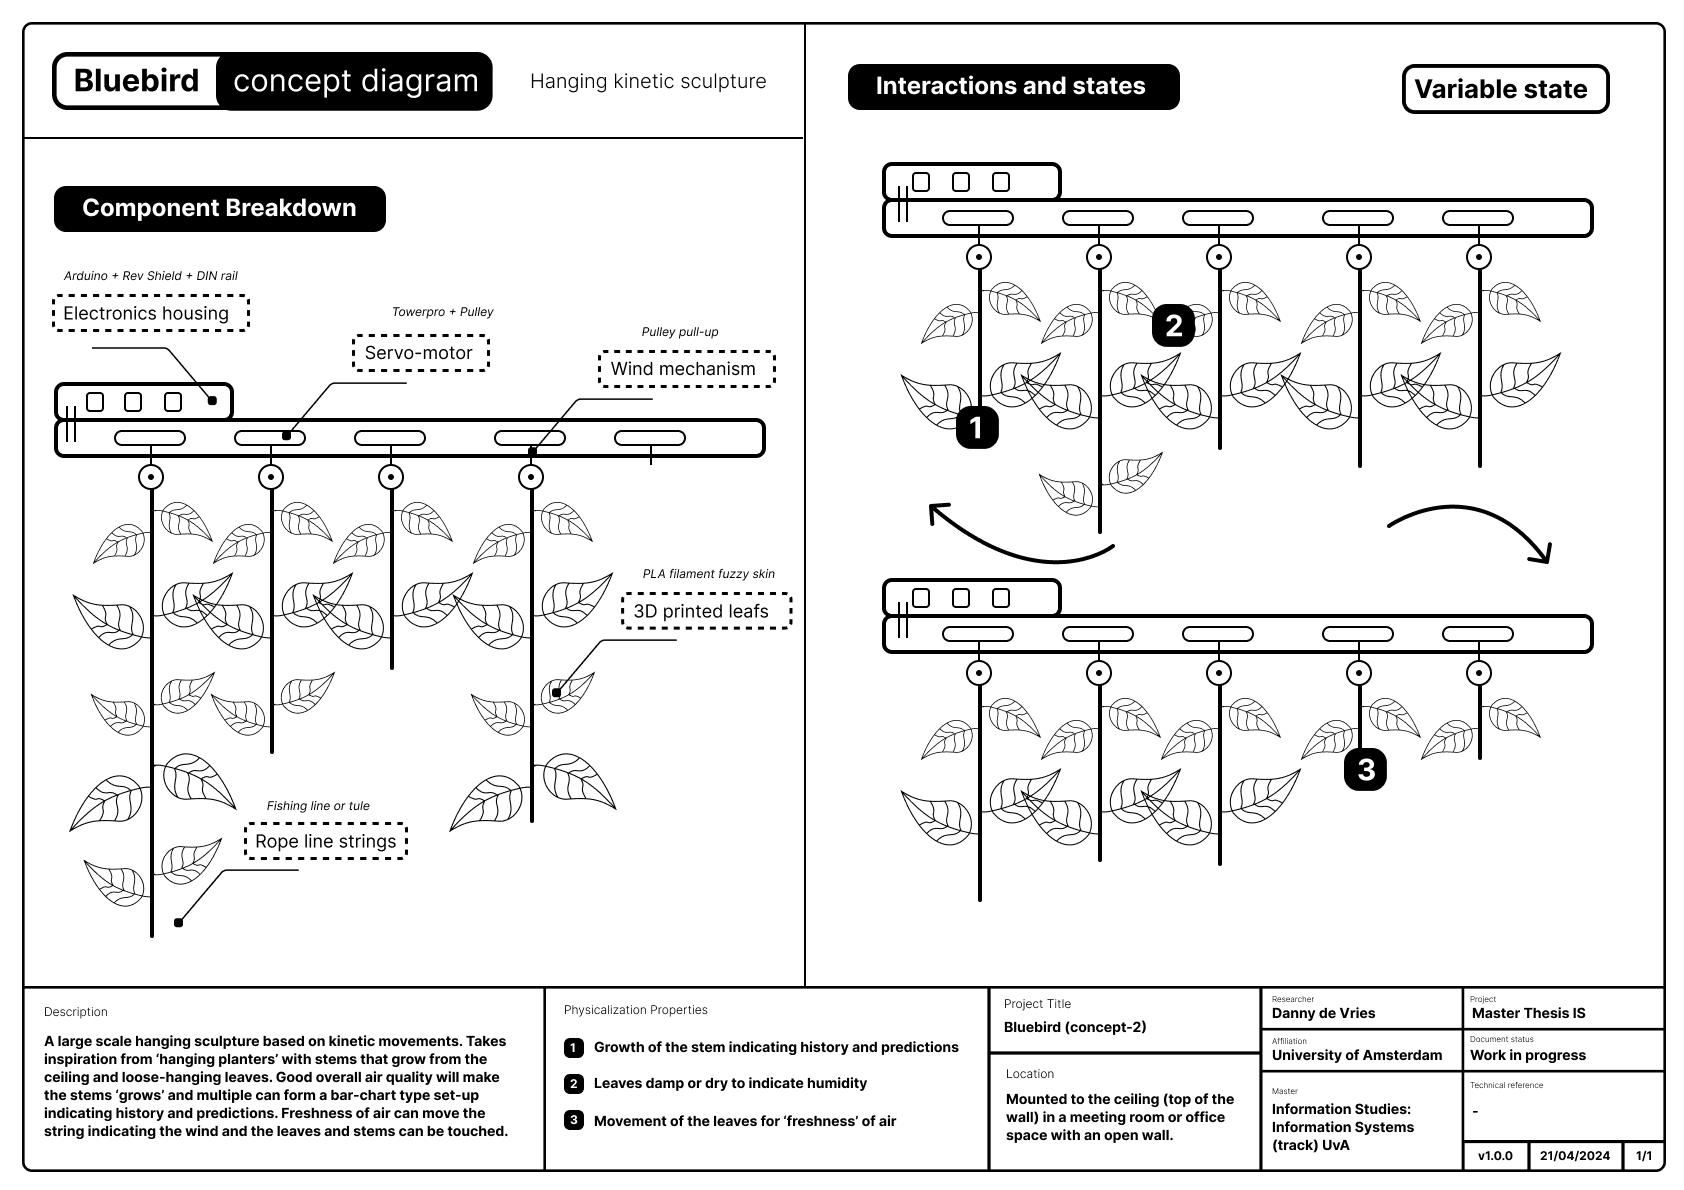
\includegraphics[width=0.6\paperwidth]{Concept-2_Bluebird_Design_Diagram.jpg}
    \caption{Design diagram of Concept-2}
    \label{fig:timeline}
\end{figure}

\begin{figure}[H]
    \centering
    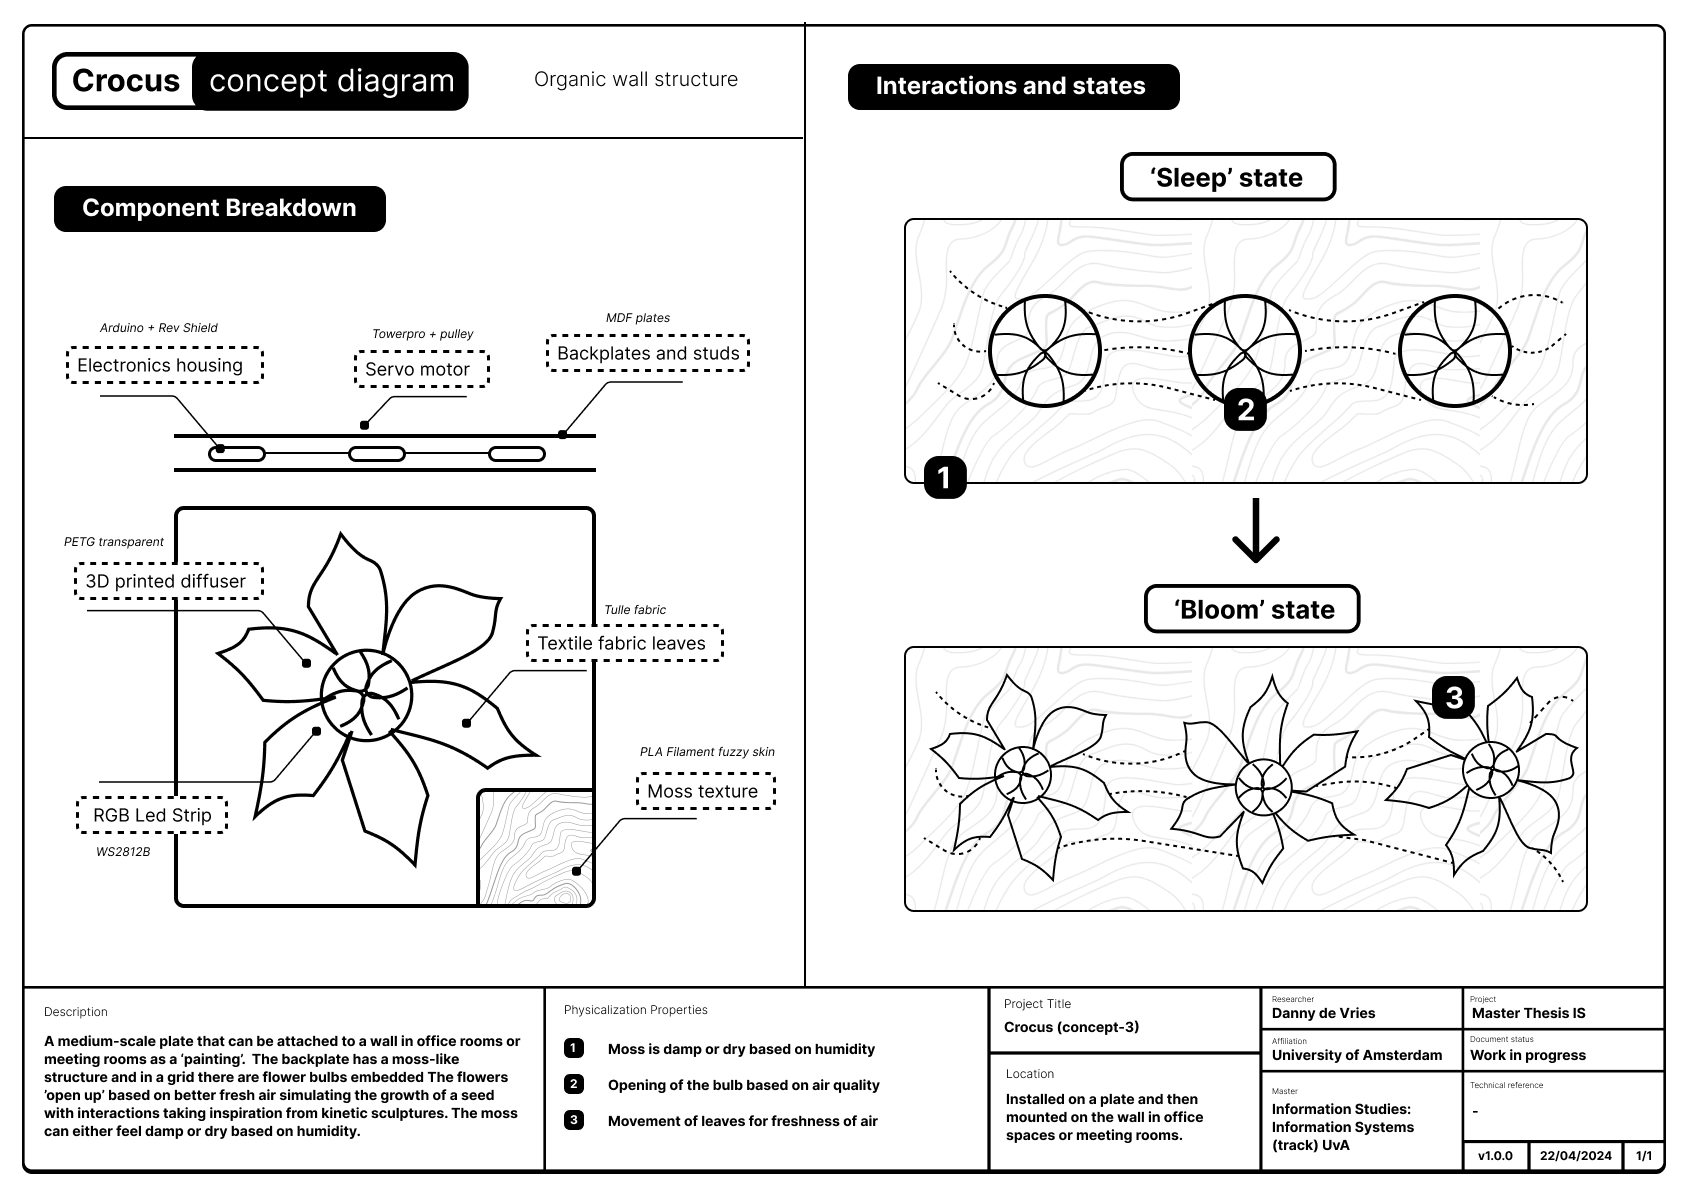
\includegraphics[width=0.6\paperwidth]{Concept-3_Crocus_Design_Diagram.jpg}
    \caption{Design diagram of Concept-3}
    \label{fig:timeline}
\end{figure}

\section{Academic sample case studies}
\label{appendix:academic}

In the ideation phase and development of concept models, seven academic publications were instrumental in informing and inspiring the design process. Table 1 provides an overview of these publications, presenting details such as the title, authors, publication year, and relevant venue.

\begin{table}[htbp]
\centering
\caption{Overview of the 7 academic case studies used for the ideation phase and concept models.}
\label{tab:my-table}
\begin{tabularx}{\textwidth}{|>{\raggedright\arraybackslash}m{1cm}|X|X|>{\raggedright\arraybackslash}m{1cm}|X|X|}
\hline
\textbf{Nr.} & \textbf{Sample} & \textbf{Author(s)} & \textbf{Year} & \textbf{Venue} & \textbf{Reference} \\ \hline
1 & Econundrum & Unknown & Unknown & non-academic & \href{https://dl.acm.org/doi/10.1145/3357236.3395509}{Econundrum} \\ \hline
2 & Caimform & Unknown & Unknown & non-academic & \href{http://dataphys.org/list/cairnform-a-physical-ring-chart-showing-renewable-energy-data/}{Caimform} \\ \hline
3 & Dataponics & Unknown & Unknown & non-academic & \href{http://dataphys.org/list/dataponics-human-vegetal-play/}{Dataponics} \\ \hline
4 & Garden of Eden & Unknown & Unknown & non-academic & \href{http://dataphys.org/list/garden-of-eden/}{Garden of Eden} \\ \hline
5 & Pudica & Unknown & Unknown & non-academic & \href{https://trackr-media.tangiblemedia.org/publishedmedia/Papers/715-MTA0N/Published/PDF}{Pudica} \\ \hline
6 & ComfortBox & Hamed S. Alavi et al. & 2017 & IFIP & \href{https://doi.org/10.1007/978-3-319-67687-6_16}{ComfortBox} 
\\ \hline
7 & ComFeel & Ugo Sassi et al. & 2020 & ACM & \href{https://dl.acm.org/doi/10.1145/3432234}{ComFeel} 
\\ \hline
8 & WindowWall & Patrick Bader et al. & 2020 & ACM & \href{https://doi.org/10.1145/3310275}{WindowWall} \\ \hline
9 & Ambient Influence & Yvonne Rogers et al. & 2010 & ACM & \href{https://dl.acm.org/doi/10.1145/1864349.1864372}{Ambient Influence} 
\\ \hline
10 & Hilo-wear & Shailin Zong et al. & 2020 & CHI & \href{https://dl.acm.org/doi/10.1145/3334480.3382813}{Hilo-wear} 
\\ \hline
\end{tabularx}
\end{table}

\section{Non-academic sample case studies}
\label{appendix:nonacademic}

In the ideation phase and development of concept models, an exploration of non-academic case studies were instrumental in informing and inspiring the design process. Table 2 presents an overview of the 15 non-academic case studies. Each entry in the table includes essential details such as the title, creator, publication year, and a brief description of the case study's venue.

\begin{table}[htbp]
\centering
\caption{Overview of the 28 non-academic case studies used for the ideation phase and concept models.}
\label{tab:my-table}
\begin{tabularx}{\textwidth}{|>{\raggedright\arraybackslash}m{1cm}|X|X|>{\raggedright\arraybackslash}m{1cm}|X|X|}
\hline
\textbf{Nr.} & \textbf{Sample} & \textbf{Creator} & \textbf{Year} & \textbf{Venue} & \textbf{Reference} \\ \hline
1 & Birdie Design & Birdie Design & 2024 & non-academic & \href{https://www.bir.die/}{www.bir.die} \\ \hline
2 & Fields of Informality & Zhestkov & 2024 & non-academic & \href{https://www.artco.m.com/}{www.artco.m} \\ \hline
3 & Tree of Ténéré & Studio Drift & 2024 & non-academic & \href{https://studiodr.ift.com/}{www.studiodr} \\ \hline
4 & Kinetic Sculpture & ART+COM & 2024 & non-academic & \href{https://artco.m.com/}{www.artco.m} \\ \hline
5 & Electro Magnetic Field & Unknown & 2024 & non-academic & - \\ \hline
6 & Microsurgical Robot & Unknown & 2024 & non-academic & - \\ \hline
7 & Wind 3.0 & Studio Roosegaarde & 2024 & non-academic & \href{https://www.studior.oo/}{www.studior} \\ \hline
8 & Floralis Generica & Eduardo Catalano & 2024 & non-academic & - \\ \hline
9 & Lucid Stead & Phillip K. Smith III & 2024 & non-academic & - \\ \hline
10 & Flylight & Studio Drift & 2024 & non-academic & - \\ \hline
11 & Spectra 2 & FIELD & 2024 & non-academic & - \\ \hline
12 & Meadow & Studio Drift & 2024 & non-academic & - \\ \hline
13 & Wind Pavilion & Studio Roosegaarde & 2024 & non-academic & - \\ \hline
14 & Pet Lamp & Álvaro Catalán & 2024 & non-academic & - \\ \hline
15 & Living map & Unknown & Unknown & non-academic & \href{https://www.behance.net/gallery/68572509/LIVING-MAP}{Living map} \\ \hline
16 & Harassment plants & Unknown & Unknown & non-academic & \href{https://luizaugustomm.github.io/pages/harassment-plants.html}{Harassment plants} \\ \hline
17 & Popsicles of Pollution & Unknown & Unknown & non-academic & \href{https://www.theguardian.com/cities/gallery/2017/sep/01/popsicles-pollution-ice-lollies-taiwan-taipei-contaminated-waterways}{Popsicles of Pollution} \\ \hline
18 & Yellow Dust & Unknown & Unknown & non-academic & \href{http://yellowdust.intheair.es/}{Yellow Dust} \\ \hline
19 & Touching air & Unknown & Unknown & non-academic & \href{https://www.stefanieposavec.com/airtransformed}{Touching air} \\ \hline
20 & Physical Weather Display & Unknown & Unknown & non-academic & \href{https://www.boredpanda.com/weather-forecast-box-tempescope-ken-kawamoto/}{Physical Weather Display} \\ \hline
21 & Inequalities Quipu & Unknown & Unknown & non-academic & \href{https://tuteja.info/inequalities-quipu/}{Inequalities Quipu} \\ \hline
22 & Summer in the city & Unknown & Unknown & non-academic & \href{https://www.carolabartsch.ch/en/projects/dataviz}{Summer in the city} \\ \hline
23 & WeatherWindow & Unknown & Unknown & non-academic & \href{http://dataphys.org/list/weatherwindow/}{WeatherWindow} \\ \hline
24 & Point cloud & Unknown & Unknown & non-academic & \href{https://www.jamesleng.net/pointcloud/}{Point cloud} \\ \hline
25 & Tele-present water & Unknown & Unknown & non-academic & \href{https://www.dwbowen.com/telepresentwater/}{Tele-present water} \\ \hline
26 & Real-time Warning & Unknown & Unknown & non-academic & \href{https://vimeo.com/35520114}{Real-time Warning} \\ \hline
27 & airFIELD & Unknown & Unknown & non-academic & \href{http://dataphys.org/list/ecloud-airfield-ambient-airport-visualizations/}{airFIELD} \\ \hline
28 & Shanghai Spheres & Unknown & Unknown & non-academic & \href{https://www.taittowers.com/work?sort=newest}{Shanghai Spheres} \\ \hline
\end{tabularx}
\end{table}

\section{fabrication Techniques}
\label{appendix:fabrication}

\begin{table}[!htbp]
\centering
\caption{Overview of the 4 academic and 6 non-academic sample case studies used as inspiration for fabrication of the prototype.}
\label{tab:my-table}
\begin{tabularx}{\textwidth}{|>{\raggedright\arraybackslash}m{1cm}|X|X|>{\raggedright\arraybackslash}m{1cm}|X|X|}
\hline
\textbf{Nr.} & \textbf{Sample} & \textbf{Author(s)} & \textbf{Year} & \textbf{Venue} & \textbf{Reference} \\ \hline
1 & FibeRobo & Jack Forman et al. & 2023 & MIT Media Lab (TGM) & \href{https://trackr-media.tangiblemedia.org/publishedmedia/Papers/728-MTA2O/Published/PDF}{TGM} \\ \hline
2 & DefeXtiles & Jack Forman et al. & 2020 & MIT Media Lab (TGM) & \href{https://trackr-media.tangiblemedia.org/publishedmedia/Papers/703-MTAyN/Published/PDF}{TGM} \\ \hline
3 & Cilllia & Jifei Ou et al. & 2016 & MIT Media Lab (TGM) & \href{https://trackr-media.tangiblemedia.org/publishedmedia/Papers/703-MTAyN/Published/PDF}{TGM} \\ \hline
4 & UniMorph & Felix Heiberg et al. & 2015 & MIT Media Lab (TGM) & \href{https://trackr-media.tangiblemedia.org/publishedmedia/Papers/703-MTAyN/Published/PDF}{TGM} \\ \hline
5 & Geometric Floating Fabric & Billie Ruben & 2020 & non-academic & \href{https://www.printables.com/en/model/42342-geometric-floating-fabric-printed-necklace-by-bill}{Printables} \\ \hline
6 & Print On Fabric & Damien Jorrand & 2021 & non-academic & \href{https://than.gs/m/14347}{Thangs} \\ \hline
7 & Nasa Fabric Mk3 & John Bowler & 2018 & non-academic & \href{https://www.thingiverse.com/thing:3095799}{Thingiverse} \\ \hline  
8 & Servo Flower & Job Smolders & 2018 & non-academic & \href{https://pinshape.com/items/41182-3d-printed-servo-flower}{Pinshape} \\ \hline
9 & Multiuse Flexible Fabric & Posix & 2024 & non-academic & \href{https://www.printables.com/model/88579-multiuse-flexible-fabric}{Printables} \\ \hline
10 & Leaf Decorative Holder & Trilobyte3D & 2022 & non-academic & \href{https://www.printables.com/model/230363-leaf-drink-coasters-with-decorative-plant-holder}{Printables} \\ \hline
\end{tabularx}
\end{table}

\end{appendices}